\section{Tracking}
\label{sec:tracking}
This section describes the performance of ITS-only tracking. During the 13def and 17q periods, the TPC was either not read out or compromised due to space-charge distortions so we rely on only the ITS for track reconstruction. Thus the purpose of this section is to demonstrate that we can use ITS-only tracking to measure tracks up to relatively large track $\pt$.

Our strategy is to measure the charged-particle $\pt$-spectrum using ITS-only tracking and to compare it with the normal TPC+ITS tracking in the data-taking period when the TPC was active and free of space-charge distortions (i.e. the low-luminosity 13b data-taking period of 5 TeV \pPb~minimum-bias data) and with published ALICE measurements~\cite{Acharya:2018qsh} that use the same dataset. By comparing to published measurements in the same system and center-of-mass energy, we avoid any ambiguity related to the reference spectrum. 

Our aim is to validate the combined effect of tracking efficiency, fake rate, and track momentum smearing corrections that are based on MC simulations. We also rely on this study to estimate systematic uncertainties due to mis-modeling of the tracking performance. So, in effect, we are performing a cross-calibration or bootstrapping with the standard ALICE tracking.

For this study, we use minimum bias \pPb~events for both data and Monte Carlo. The Monte Carlo simulations used for this section are LHC13b2\_efix\_p1, which a \textsc{DPMJET} anchored to LHC13b,c and LHC17l3b, which is a pp \textsc{Pythia8}, anchored to LHC17p. The data used runs from LHC13b. The \pPb~data sets match the ones used in the published ALICE measurements mentioned previously. 

For this tracking performance analysis, we  only use events with the minimum bias trigger (CINT7). We also apply the vertex and pileup selections described in Section~\ref{sec:eventselection}. The tracks reconstructed from the ITS (``ITS-only tracks"), are compared with tracks reconstructed from information obtained from both the TPC and ITS (``TPC+ITS tracks"). Here, ITS-only tracks are really reconstructed in a standalone way and are not simply the ITS-segment of a ITS+TPC track.~\footnote{The standalone ITS-only tracks can be retrieved from ESD data by demanding a track status of `` \textsc{AliESDtrack::kITSPureSA}''. The exact line in the code is a follows: \textit{        \_track\_cut.back().SetRequireITSPureStandAlone(kTRUE);}.}

In order to select good-quality tracks emerging from the primary vertex while maintaining a high efficiency, each track is required to satisfy the cuts summarized in Table~\ref{tab:track_cuts}. A set of standard PWG-JE cuts are applied to all tracks, and additional track cuts are applied depending on whether the track is a TPC+ITS track or an ITS-only track. 
\begin{table}[h]
   \centering
      \caption{Summary of the cuts used in Track Selection.}	
   \label{tab:track_cuts}
   \begin{tabular*}{1.0\columnwidth}{@{\extracolsep{\fill}}l|c@{}}
      	\hline
 		\textbf{Common Cuts}\\
        %\textbf{ITS--Only Cuts}\\
        \hline
        track $\eta$ & $|\eta| < 0.8$\\
        track $\pt$ & $\pt \geq 0.150$ \GeVc\\
        SetMaxDCAToVertexXY & 2.4 cm\\
        SetMaxDCAToVertexZ & 3.2 cm\\
        SetDCAToVertex2D & TRUE\\
		\hline \hline
        \textbf{TPC+ITS Cuts}\\
        \hline
        SetMinNClustersTPCPtDep & 70.+30./20.*x, 20.0\\ 
        SetMinNClustersTPC & 70\\
        SetMaxChi2PerClusterTPC & 4\\
        SetMaxChi2PerClusterITS & 36\\
        SetMaxFractionSharedTPCClusters & 0.4\\
        SetMaxChi2TPCConstrainedGlobal &36 \\
        SetRequireTPCStandAlone & TRUE\\
        SetRequireTPCRefit & TRUE \\
        SetRequireITSRefit & TRUE\\
        SetRequireSigmaToVertex & FALSE \\
        SetAcceptKinkDaughters & FALSE\\
        \hline \hline
        \textbf{ITS--Only Cuts}\\
        \hline
        SetRequireITSPureStandAlone &TRUE\\
        SetMinNClustersITS & 4\\
        SetMaxChi2PerClusterITS & 36\\
        \hline
   \end{tabular*}
\end{table}
\FloatBarrier
\subsection{Tracking performance with and without TPC}
\label{sec:closurewithdata}
Our strategy to validate the use of ITS-only tracking relies on cross-calibration with the normal TPC+ITS tracking and comparisons with published data. To this end, we first measure a charged-particle $\pt$ spectrum using TPC+ITS reconstruction to reproduce the published data and thus demonstrate the validity of our method. We then repeat the measurement with ITS-only reconstruction and compare the results.

The method we use contains the following steps: 
\begin{enumerate}
\item Using the MC simulations, obtain the efficiency, the fake rate, and a track-$\pt$ response matrix.
\item Obtain a $\pt$ spectrum from the minimum-bias data with either ITS-only or TPC+ITS tracking. 
\item Apply a $\pt$-dependent fake rate correction to the spectra of point 2. 
\item Multiply the published spectrum by the track efficiency. 
\item Finally, use the response matrix to smear the result of point 4.
\item Compare the result of point 5 with the result of point 3. 
\end{enumerate}

If the efficiency, fake rate, and response matrix, which are all obtained from MC simulations, faithfully represent the tracking performance of the data, then it follows that the result of point 3 should be compatible with the result of point 5. We use this fact to constrain the degree to which mis-modeling of the detector response could affect single-track $\pt$ spectra.

Note that we could have attempted to directly measure a charged-particle spectrum, applying an efficiency correction to the result of point 3 and then unfolding that result. That would have been directly comparable to the published data. However, the systematic uncertainties intrinsic to the unfolding procedure would result in relatively large systematic uncertainties, but these are unrelated to the issue we discuss here. 

We note that using the response matrix to smear the published data is a mathematically well-defined procedure (as opposed to unfolding, which requires an inversion of the response matrix subject to the statistical uncertainties of the data). Given that our aim is to test the corrections and response matrix in a robust and unambiguous way, we follow the above steps to avoid unfolding systematic uncertainties.

\subsubsection{Efficiency and fake rates}
\label{sec:Efficiency_fake_rates}
%The tracking efficiency is calculated from the minimum bias \pPb~simulation (see Table~\ref{tab:MCsamples}).
The tracking efficiency is defined as the ratio of the number of reconstructed primary particles\footnote{No special tuning of the particle type composition is performed. This typically only matters at low $\pt$ and enforces a small (percent level) correction to the out-of-the-box results.}, $N_{\mathrm{prim,rec}}(p_\mathrm{T})$, to the number of generated primary particles, $N_{\mathrm{prim,gen}}$. The truth-to-reconstructed matching is done following the standard ALICE method\footnote{The information is retrieved with the method ``track$\to$GetLabel()".}. Thus, the efficiency is defined as: 
\begin{equation}\label{eq:eff}
\epsilon (\pt^{\mathrm{true}}) = \frac{N_{\mathrm{prim,rec}}(\pt^{\mathrm{true}})}{N_{\mathrm{prim,gen}}(\pt^{\mathrm{true}})}.
\end{equation}

As the equation suggests, we use the simulated or ``truth'' transverse momentum, $\pt^{\mathrm{true}}$, for both the numerator and denominator in our efficiency. This way, we factorize out effects of efficiency from bin-migration due to momentum smearing.

The numerator of Equation~\ref{eq:eff} is restricted for charged particles with generated pseudorapidity in the range $|\eta^{\mathrm{true}}|<0.8$ and azimuth $0<\varphi^{\mathrm{true}}<2\pi$. Therefore, the correction factor accounts for both geometrical acceptance, detector inefficiencies, and dead channels.  

Fake tracks are defined as reconstructed tracks that do not match to a truth, primary particle. The fake rate is determined by taking a ratio of the number of fake tracks to the total reconstructed tracks and is parametrized as a function of the reconstructed transverse momentum of the track, $\pt^{\mathrm{reco}}$:

\begin{equation}\label{eq:fakes}
\mathrm{fake rate} (\pt^{\mathrm{reco}}) = \frac{N_{\mathrm{unmatched}}(\pt^{\mathrm{reco}})}{N_{\mathrm{all reco}}(\pt^{\mathrm{reco}})}.
\end{equation}

Figure~\ref{fig:tpcEff} shows the efficiency and the fake rates for the TPC+ITS and ITS only tracks. In both cases the efficiency grows with $\pt$ up to about 1 \GeVc~where it dips and it reaches a plateau value with no significant $\pt$ dependence. The efficiency starts at about 57$\%$ for the TPC+ITS tracks and at 70$\%$ for ITS-only tracks at 150 MeV and plateaus at 84\% and 88\% respectively. %The plateau is calculated by applying a constant fit from {2 $< \pt <$$ 20 GeV/c$}. 

The lower efficiency for the TPC+ITS tracks compared to ITS-only tracks is expected since the former requires a matching between ITS and TPC track segments, which has some inefficiency. This study shows that the matching efficiency is high at large $\pt$ but leads to substantial differences at low $\pt$.  

%The decrease in the tracking efficiency by about 2--5$\%$ in the range 1--3 \GeVc~is due to the fact that above about 1 \GeVc, tracks are almost straight and can be contained completely in the dead areas between TPC sectors or in ITS dead staves. Therefore, at high $\pt$ the efficiency is dominated by geometry and thus has a constant value.

The fake rate for the TPC+ITS tracks is less than a percent over the entire range shown. In comparison, the fake rate is larger in the ITS-only tracks. It is below 5\% up to 5 \GeVc, and it grows roughly linearly and reaches 15\%  at 10 \GeVc. The higher fake rate is due to the much lower number of clusters associated with ITS-only tracks (maximum of 6) than to TPC+ITS tracks (minimum of 70).
\begin{figure}[h]
\center
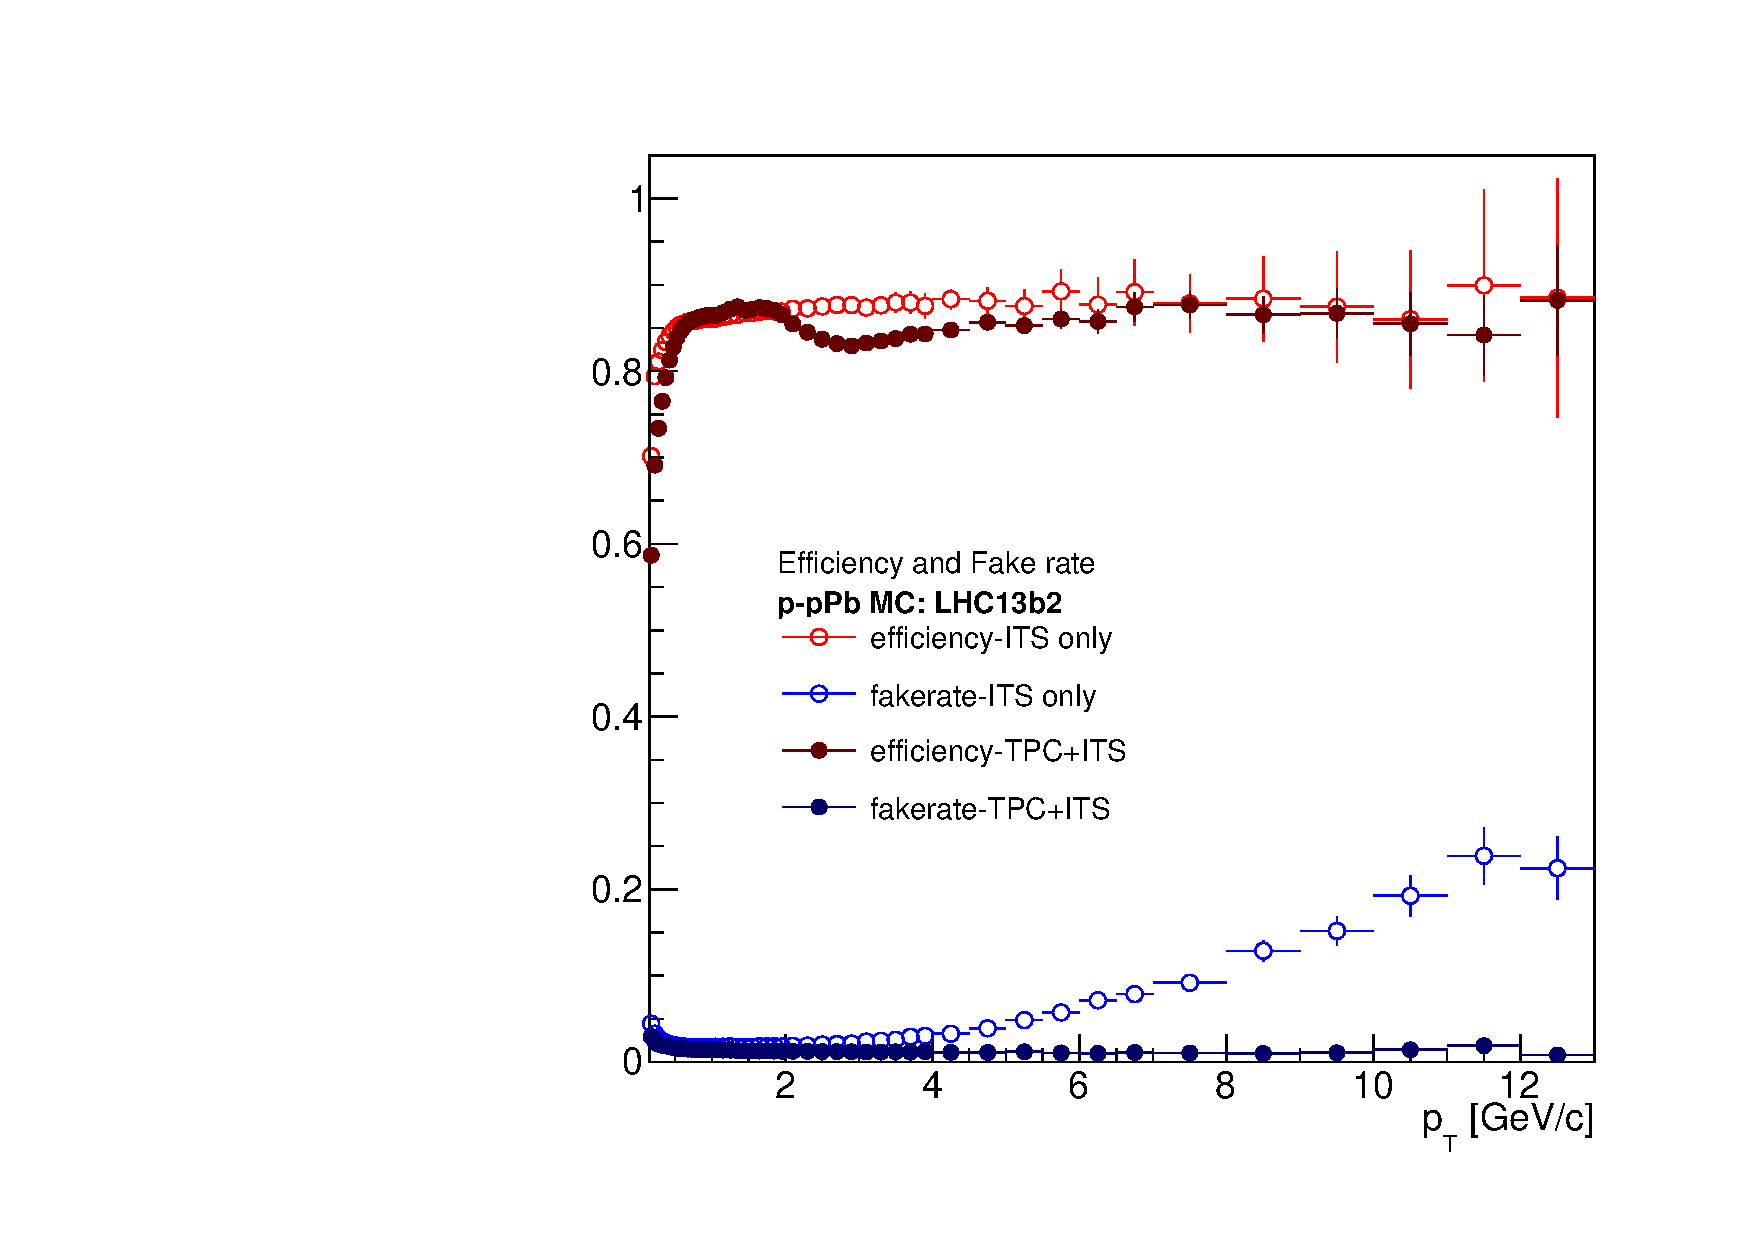
\includegraphics[width=0.5\textwidth]{Data_Analysis/Tracking/HybridAndITS_Eff_fakerate_pPb_lowpt.pdf}
\caption{Efficiency and fake rate for combined TPC+ITS tracking (filled circles) and ITS-only tracking (open circles) obtained with \pPb~simulation. The error bars represent statistical uncertainty only.}
\label{fig:tpcEff}
\end{figure}

%The efficiency and fake rate between pp and \pPb~are rather similar. Figure~\ref{fig:ppPb_eff} shows the comparison between the pp efficiency and \pPb~efficiency as well as the fake rate for pp and the fake rate for \pPb~for ITS-only tracks. The pp efficiency was calculated using the 17l3b Monte Carlo simulation. %The pp efficiency plateaus at 85\%, while the \pPb~efficiency is 88\% as mentioned previously. 
%\begin{figure}[h]
%\center
%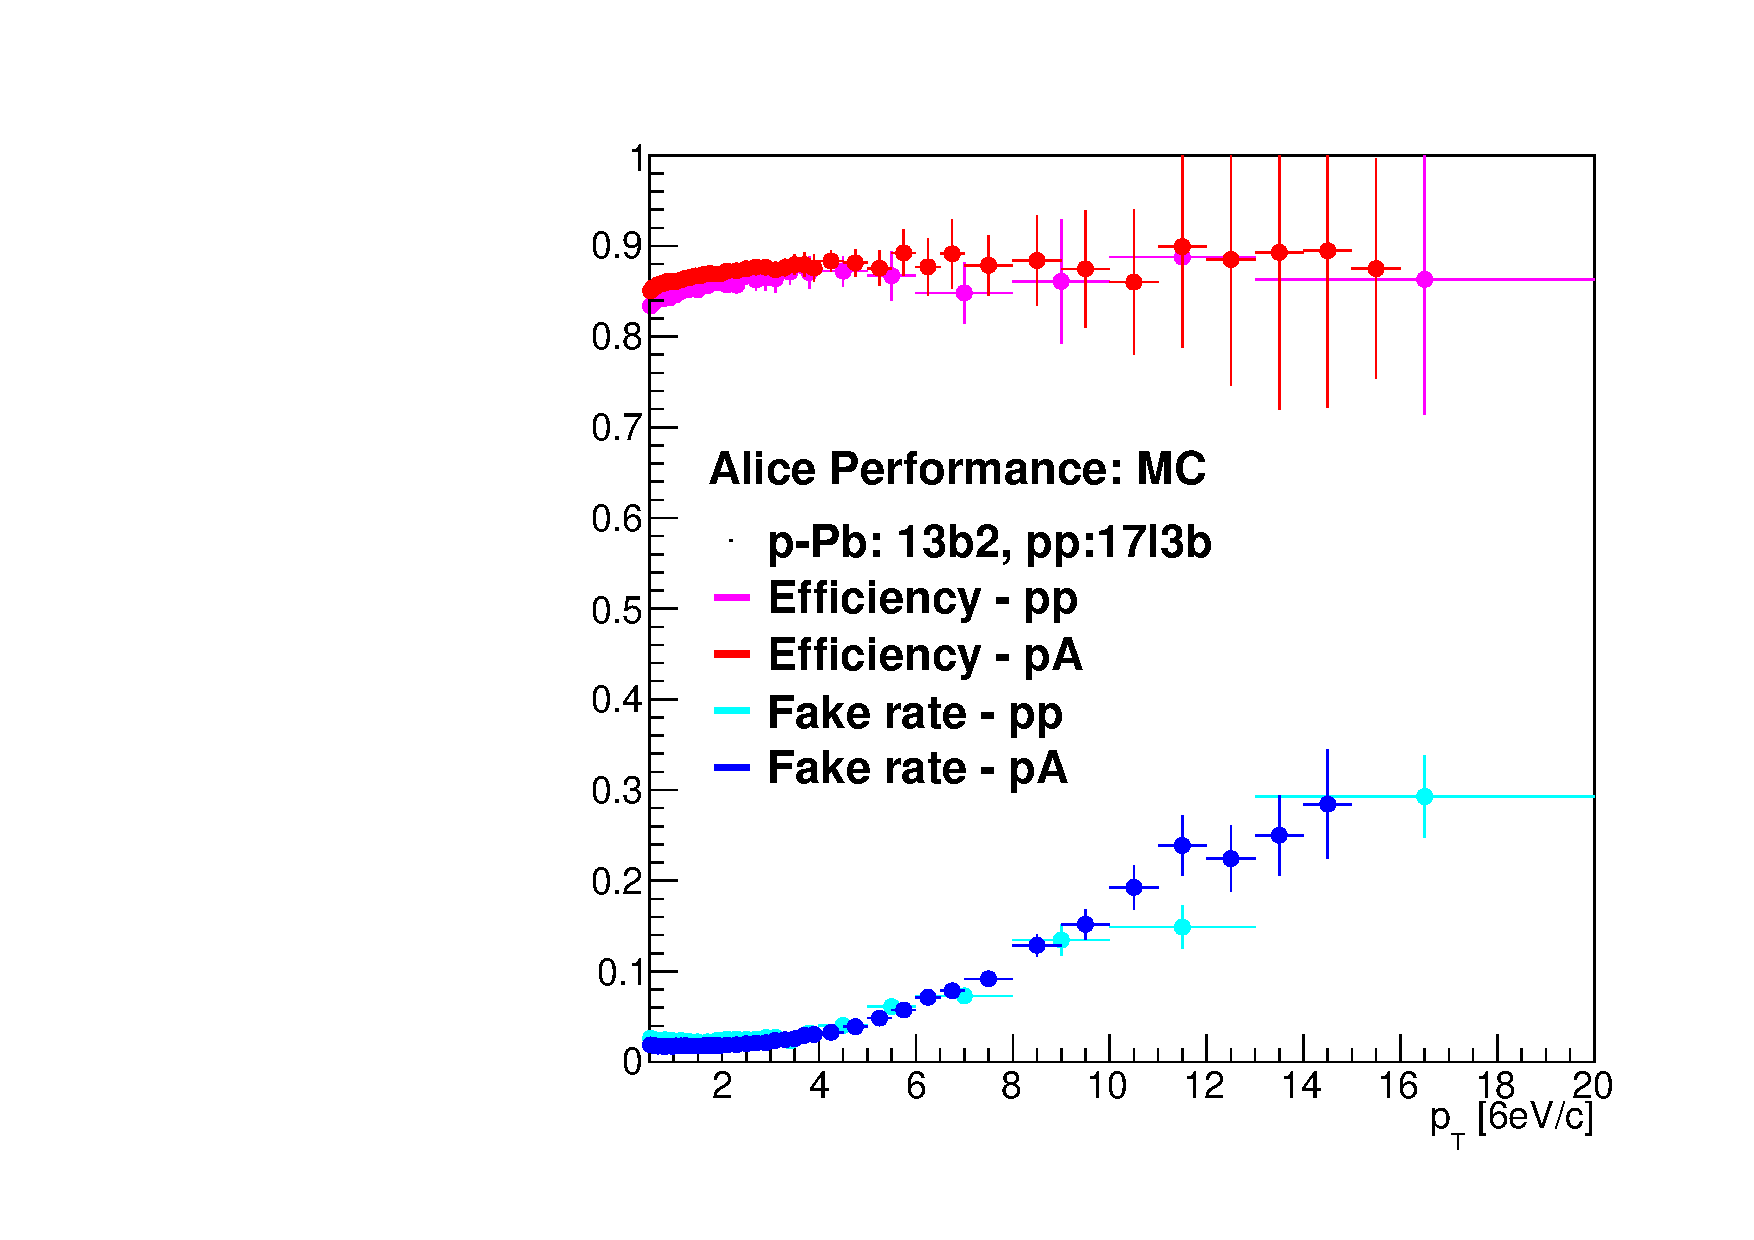
\includegraphics[width=0.7\textwidth]{Tracking/EfficiencyFakeRate_tracking_pApp_compare_halfGeV20GeV_publishedBinning.pdf}
%\caption{Efficiency and fake rate comparison between pp and \pPb~ITS-only tracks. The error bars represent statistical uncertainty only. }
%\label{fig:ppPb_eff}
%\end{figure}


\FloatBarrier

\subsubsection{Resolution, response matrix and bin migration}
The main difference between TPC+ITS and ITS-only tracking lies in the much worse momentum resolution of the latter. This is driven by geometry 
and $\int Bdl$ as the TPC covers up to {$z=$258 cm} but the ITS only to {$z=$48 cm}. 

Figure~\ref{fig:resolution} shows the momentum resolution as a function of $\pt^{\mathrm{true}}$ for 
TPC+ITS and ITS-only tracks. The momentum resolution of both increases with \pt; however, the resolution for TPC+ITS never exceeds a relative 2\% below 20 \GeVc, while the ITS-only tracking resolution is about a factor of 7 worse and reaches $\sim$15\% by 10 \GeVc. In both cases the resolution curves have the expected shape: the growth at low momentum is due to multiple-scattering and the linear growth at higher $\pt$ arises from the number and depth of position measurements, and the track bend at the measurement planes. 
\begin{figure}[h]
\center
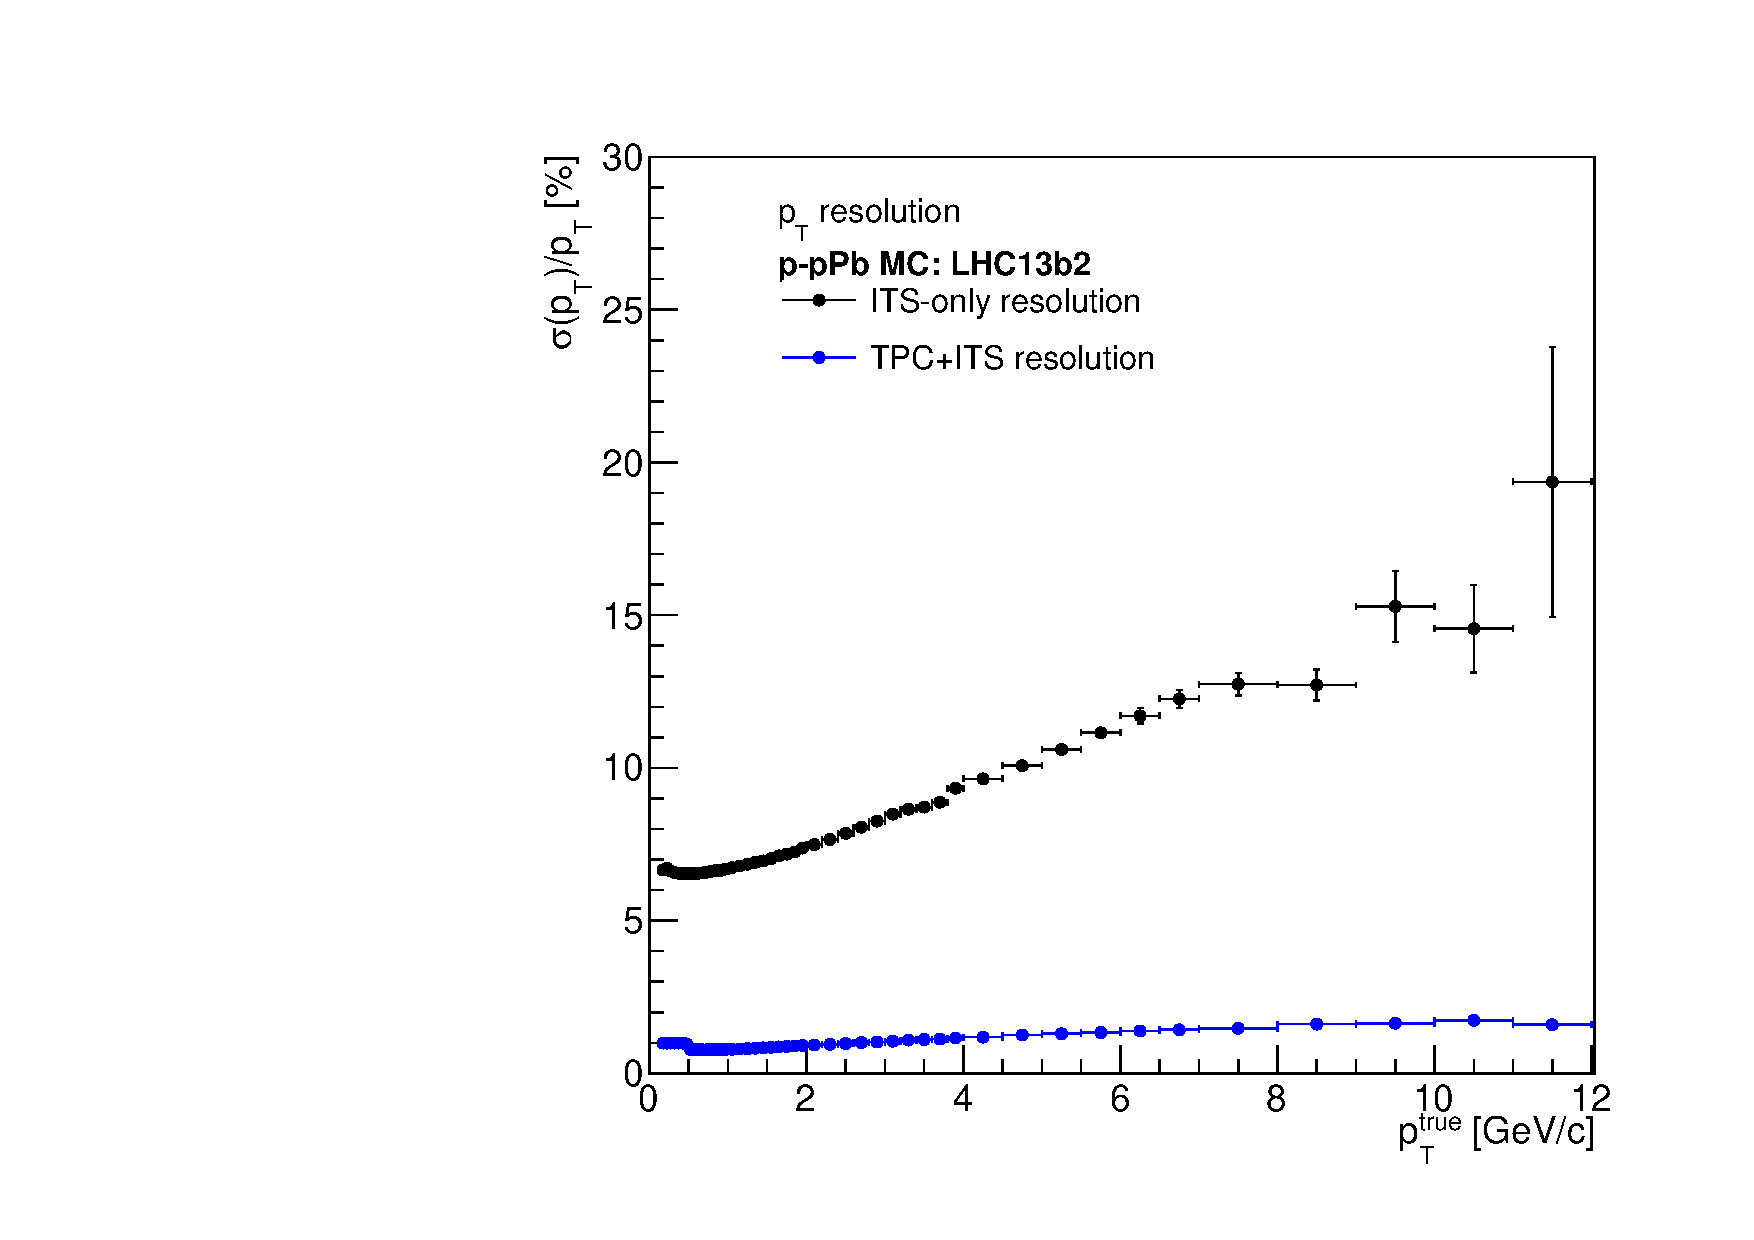
\includegraphics[width=0.5\textwidth]{Data_Analysis/Tracking/HybridAndITS_resolution_lowpt.pdf}\\
\caption{The relative $\pt$ resolution for TPC+ITS tracking and ITS only tracking. The error bar represents statistical uncertainty only.}
\label{fig:resolution}
\end{figure}

We define the tracking response matrix as the correlation between the reconstructed and the generated transverse momentum. This matrix is filled only for reconstructed tracks with a true match; fake tracks are explicitly excluded. Figure~\ref{fig:responseMatrixTPC} shows the response matrix, its one-dimensional projections, and the ratio of true to reconstructed spectra. The ratio of the true to reconstructed spectra is used to correct of the bin migration effects:

\begin{equation}\label{eq:bin_migration}
\mathrm{bin\:migration} (\pt^{\mathrm{reco}}) = \frac{N_{\mathrm{prim,reco}}(\pt^{\mathrm{true}})}{N_{\mathrm{prim,reco}}(\pt^{\mathrm{reco}})}.
\end{equation}

\begin{figure}[h!]
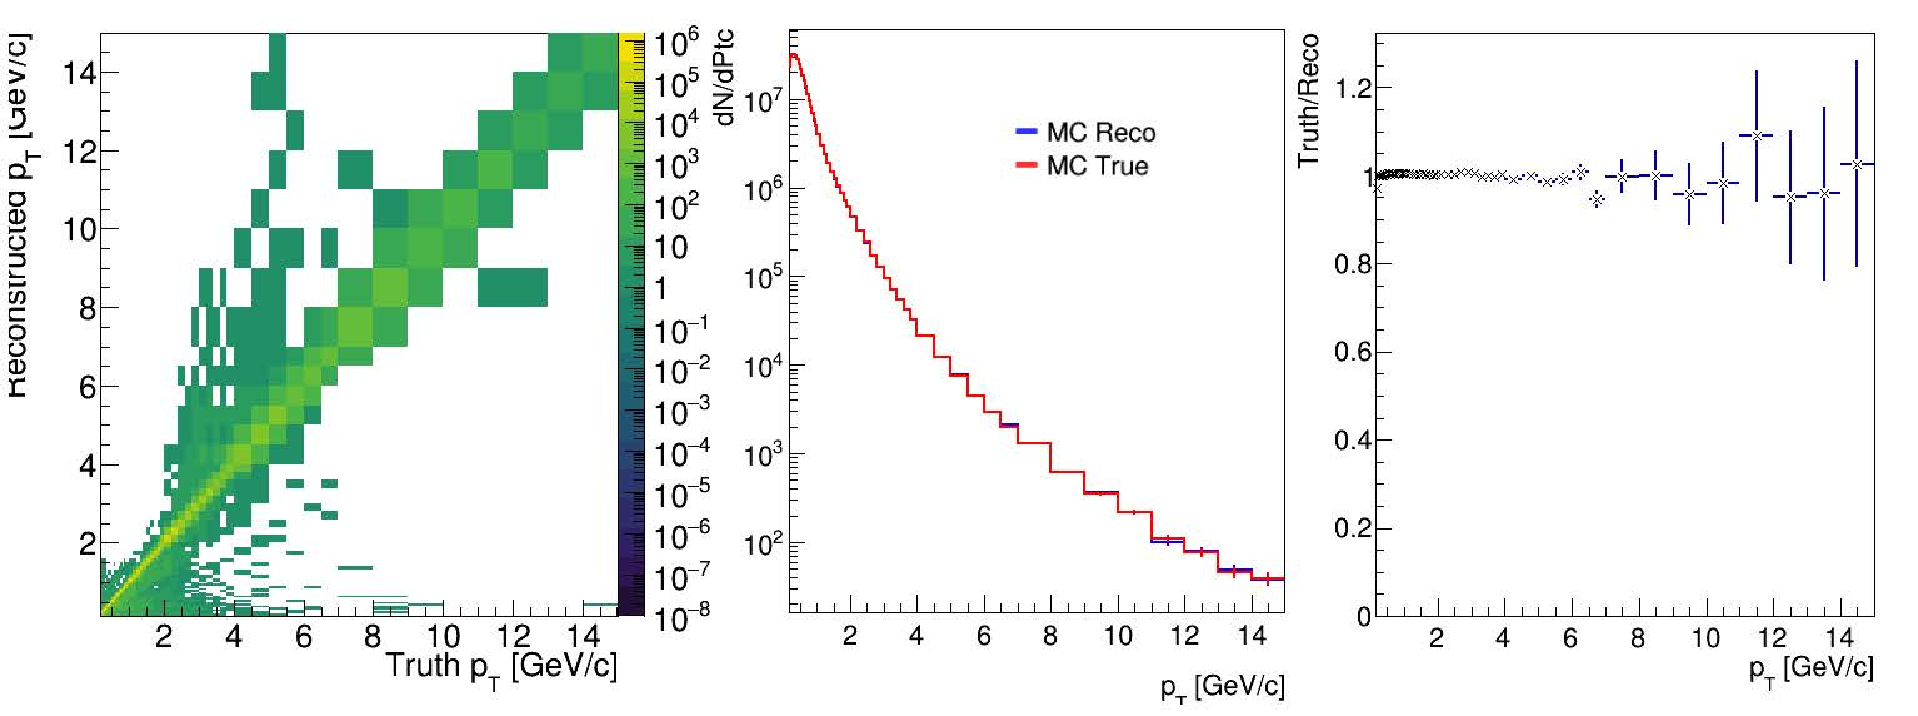
\includegraphics[width=0.965\textwidth]{Data_Analysis/Tracking/Matrix_tracking_tpc_MBMC_0GeV15GeV_dNdPt.pdf}\\
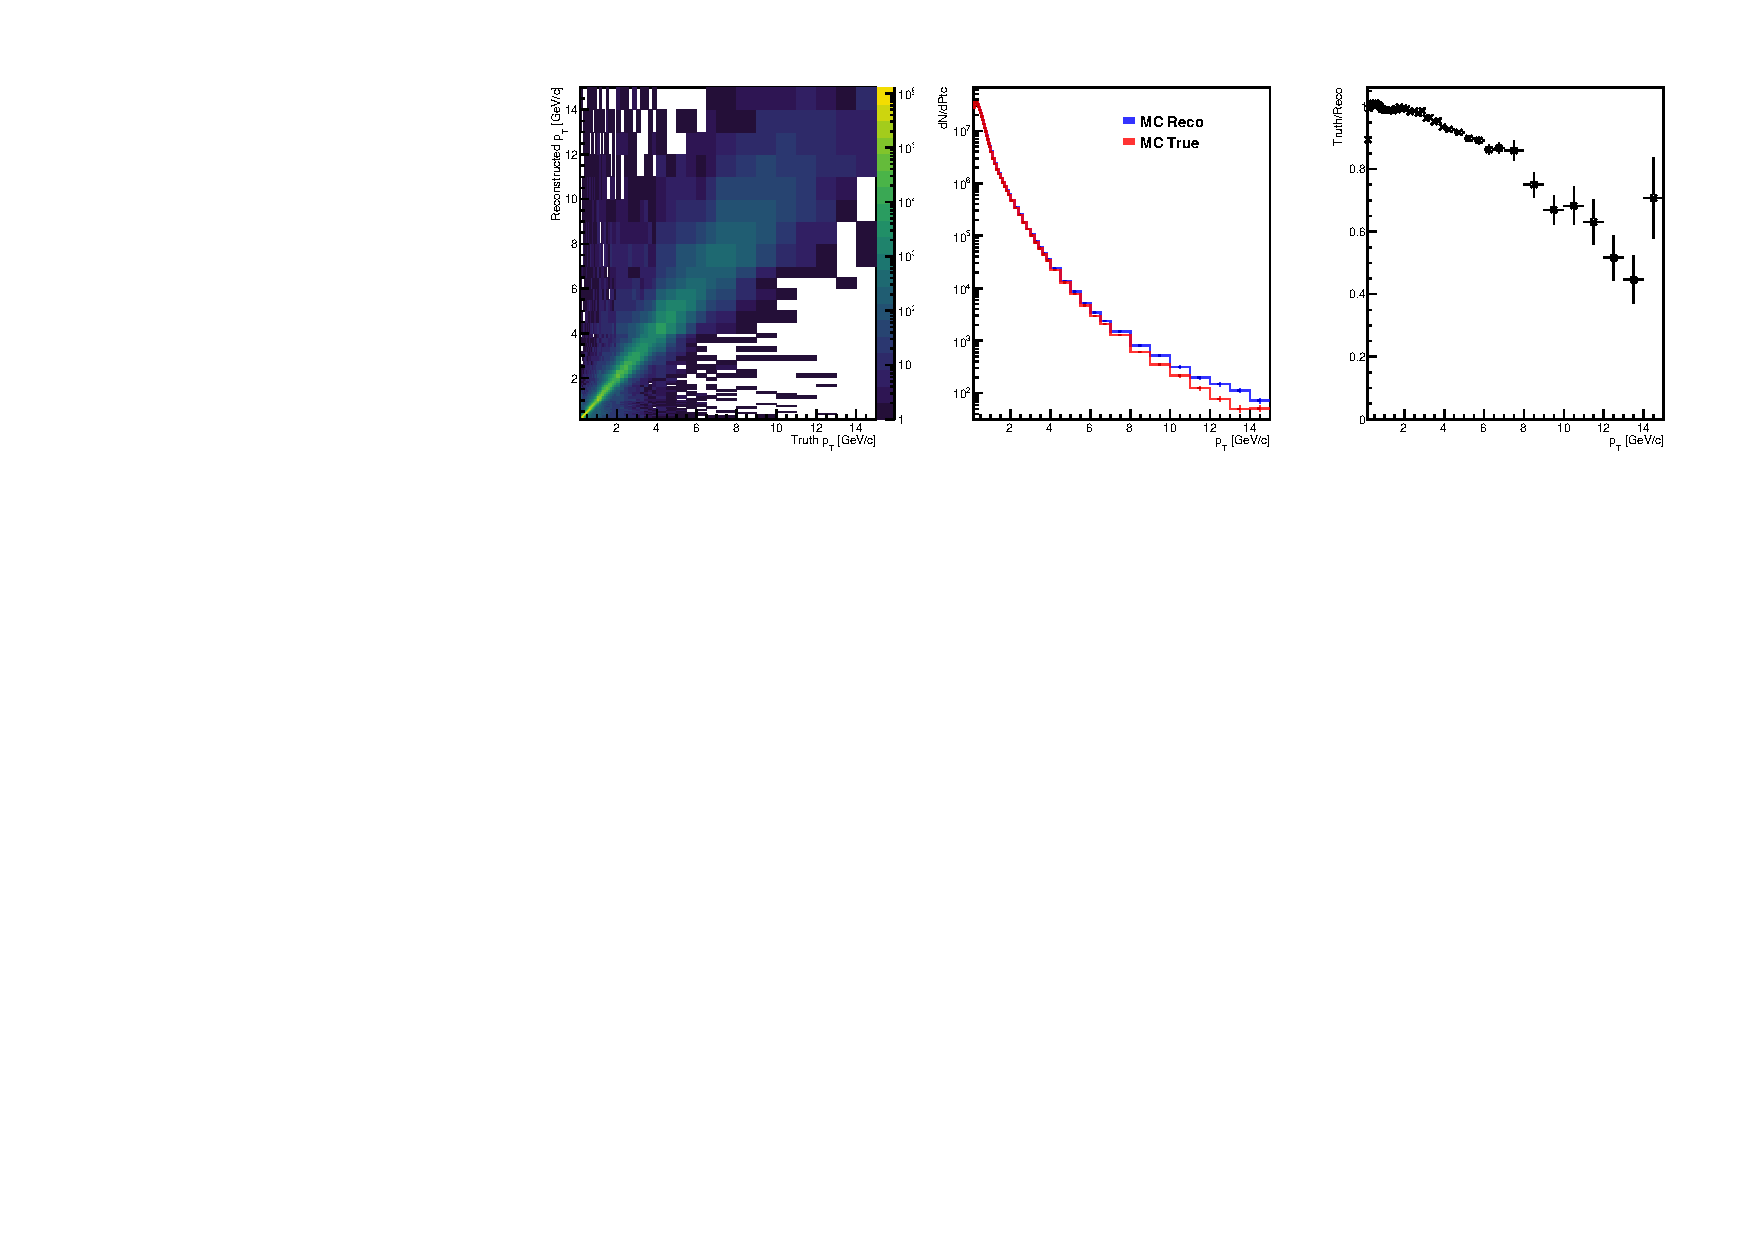
\includegraphics[width=1.0\textwidth]{Data_Analysis/Tracking/Matrix_tracking_its_MBMC_0GeV15GeV_dNdPt.pdf}

\caption{Left panel: correlation matrix between true $\pt$ and reconstructed $\pt$ of tracks reconstructed with TPC+ITS (upper row) and ITS-only (bottom row). Middle panel: projections of the response matrix into the true and reconstructed $\pt$. Right panel: ratio of true to reconstructed spectra. This ratio used as part of the bin-by-bin correction factors.}
\label{fig:responseMatrixTPC}
\end{figure}

The effect of the track momentum smearing in the ITS is clearly visible in the projection plots, where the reconstructed spectrum is significantly harder at high $\pt$. The ratio of truth to reconstructed $\pt$ is very close to unity in the TPC+ITS case, as expected. On the other hand, the ratio deviates significantly from unity in the ITS-only case; it reaches 0.9 at 6 \GeVc~and drops quickly, reaching 0.5 at about 13 \GeVc. The quick drop at high $\pt$ comes mainly from the linear degradation of the relative momentum resolution combined with the fast drop of the true spectrum to produce large effects in the tails. 

The bin migration (b), along with the tracking efficiency ($\epsilon$) and the fake rate (f) are used as the correction factor equation~\ref{eq:track_weight} for the charged hadron tracks; all of them are shown together in Figure~\ref{fig:correctionFactors}. Based on overlapping plot of pp and \pPb, we can see that correction factors are similar for tracks from a pp collision or a \pPb~collision. We conclude that the multiplicity in \pPb~is low enough such that it does not affect tracking performance.  

\begin{equation}\label{eq:track_weight}
w = \frac{1}{\epsilon}(1-f)b
\end{equation}

\begin{figure}[h]
\center
%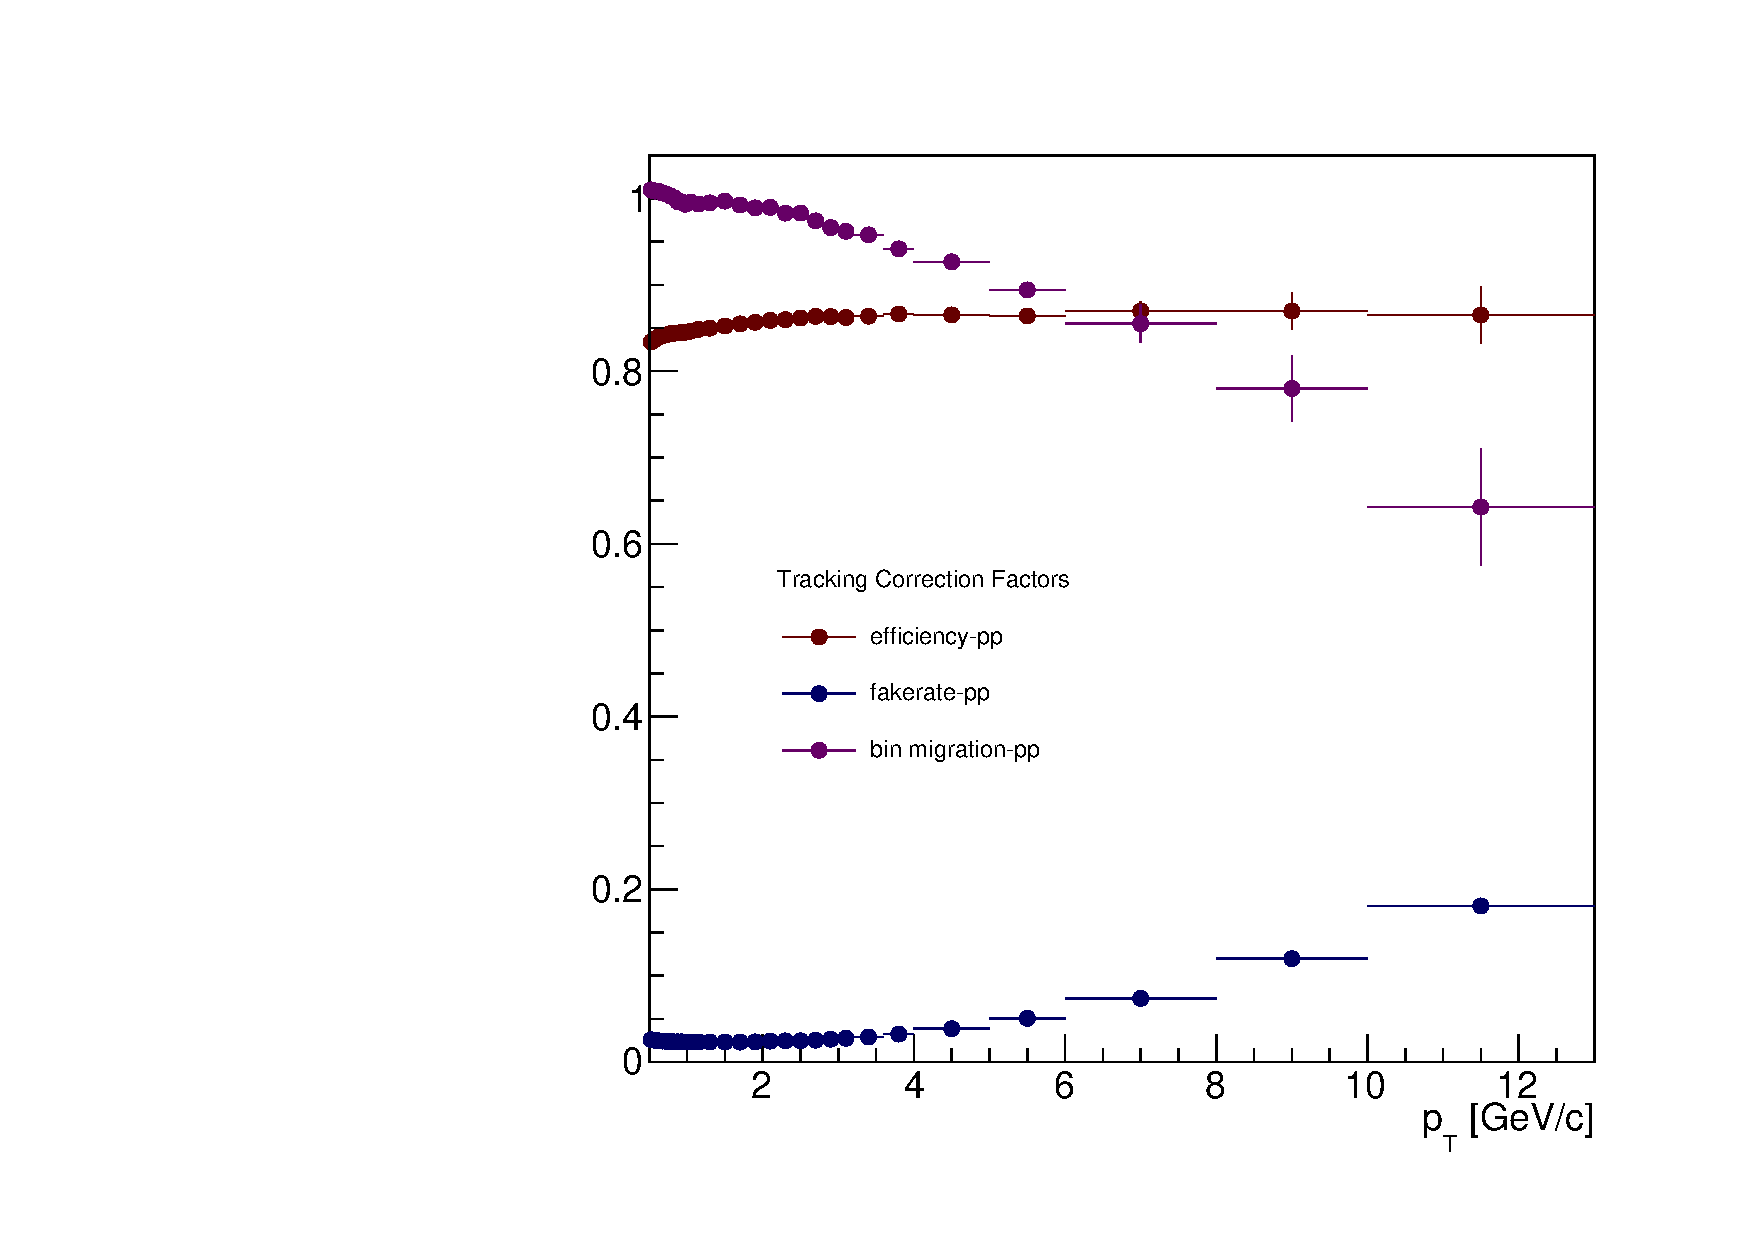
\includegraphics[width=.45\textwidth]{Data_Analysis/Tracking/trackCorrectionFactors_pp.pdf}
%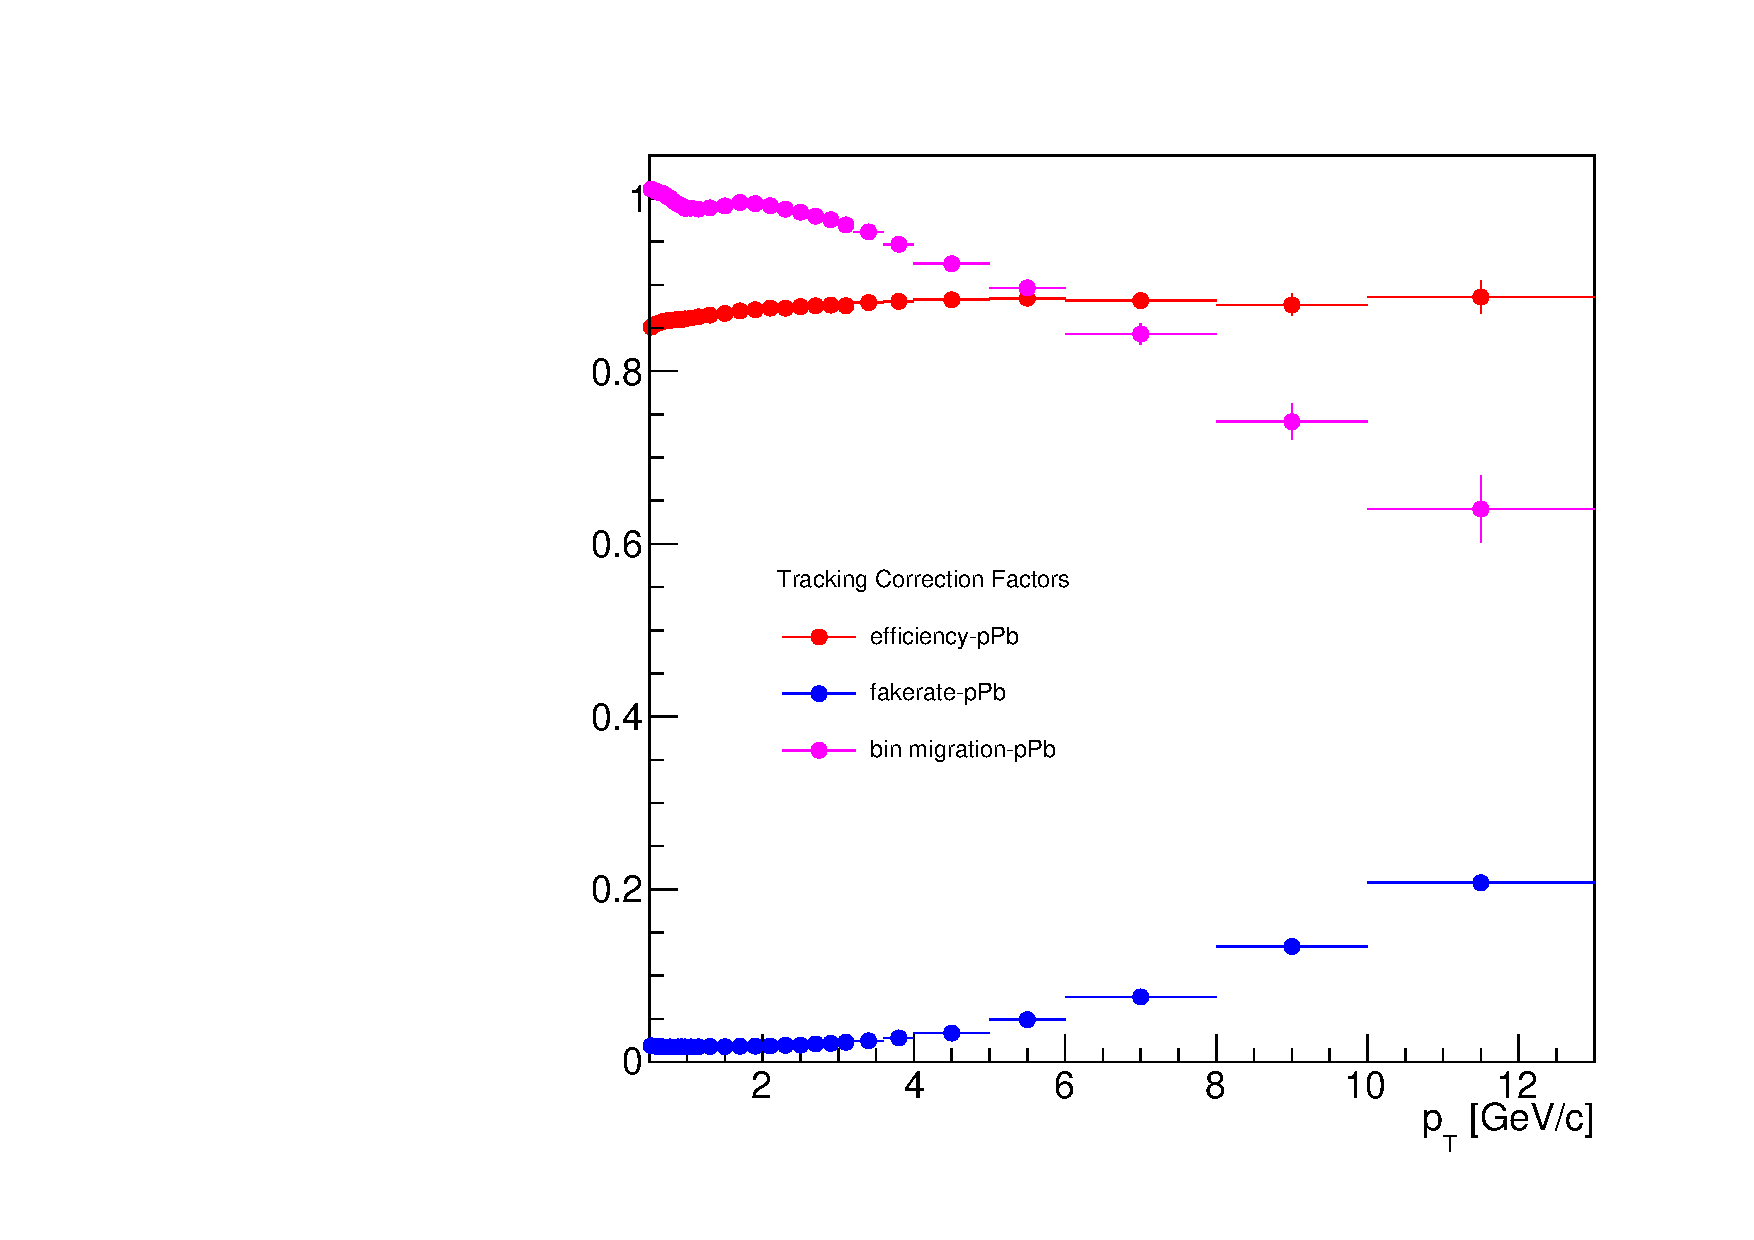
\includegraphics[width=.45\textwidth]{Data_Analysis/Tracking/trackCorrectionFactors_pPb.pdf}
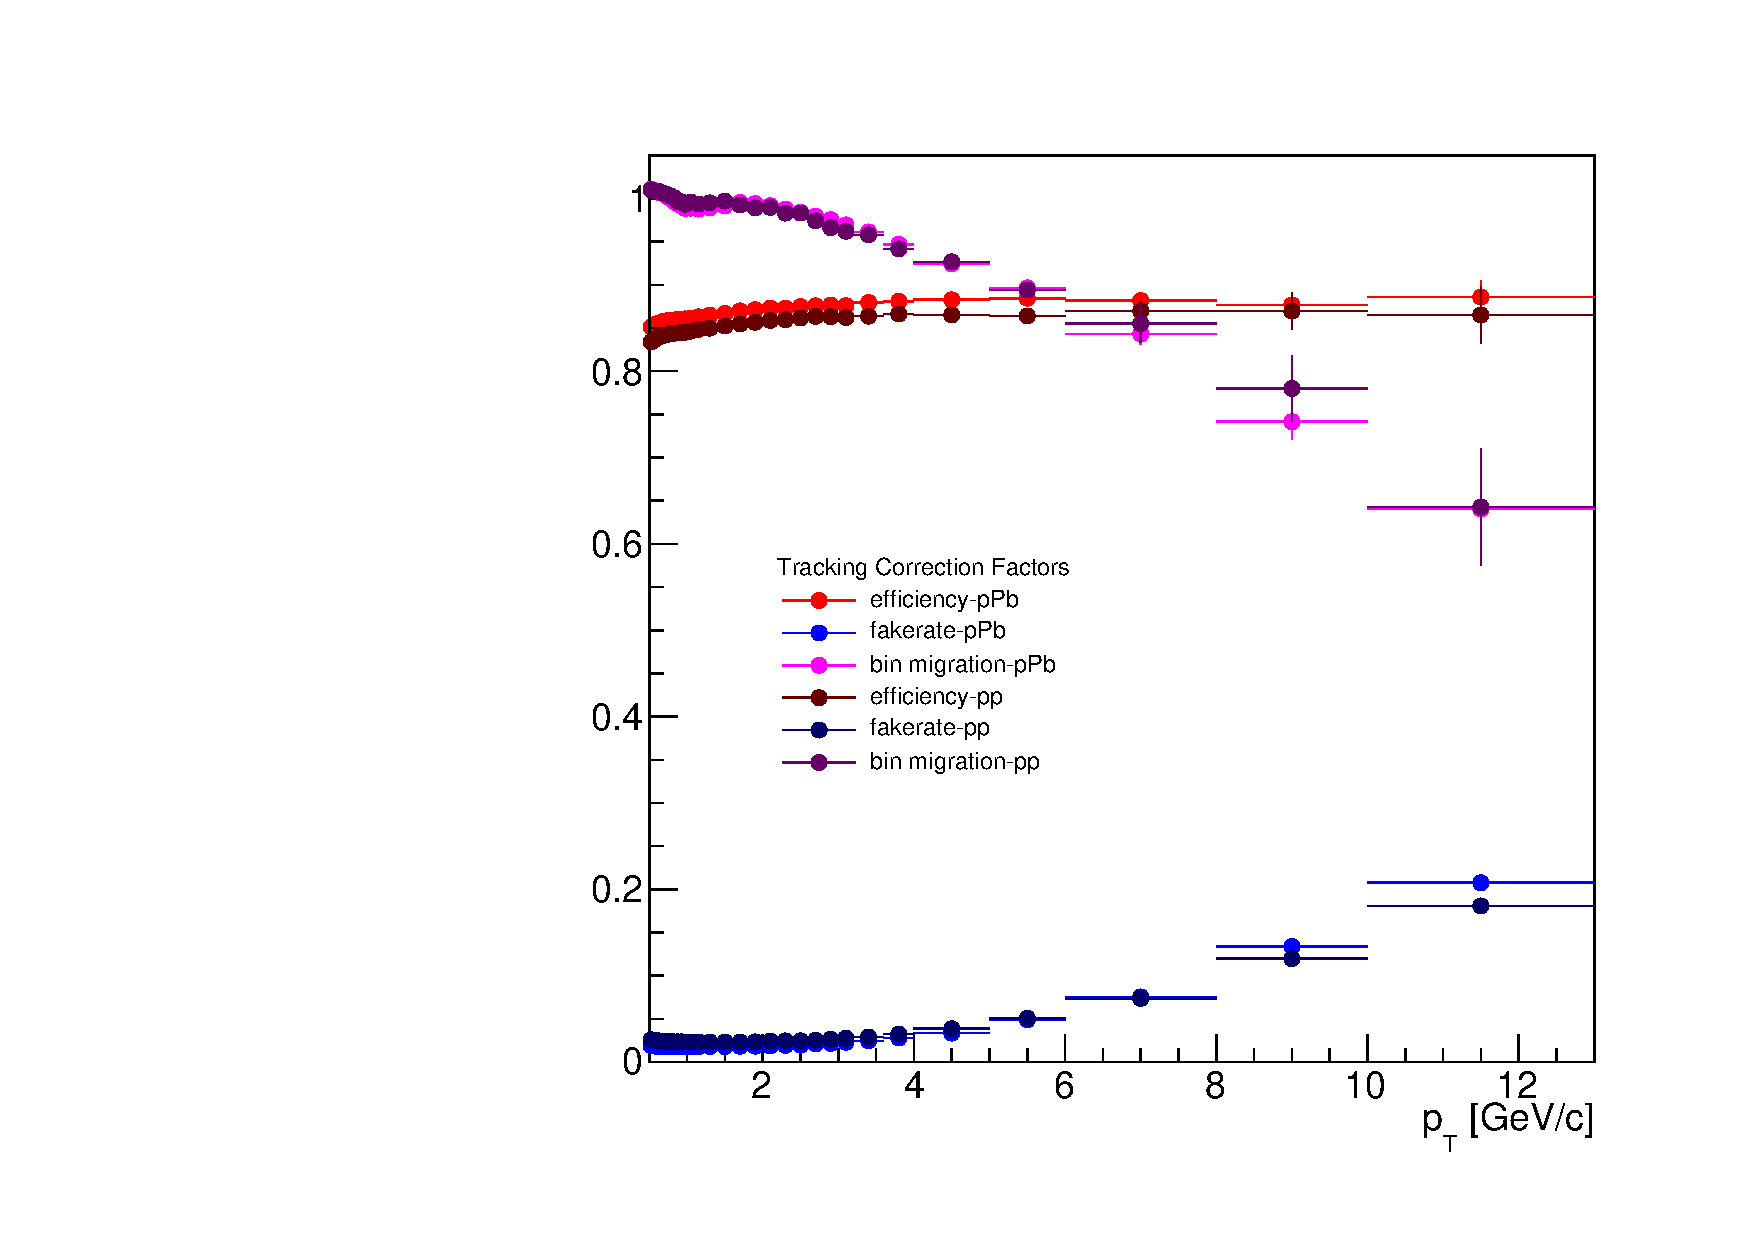
\includegraphics[width=.5\textwidth]{Data_Analysis/Tracking/trackCorrectionFactors_pPbAndpp.pdf}
\caption{The efficiency, fake rate, and momentum smearing correction factors for pp and \pPb~data.}
\label{fig:correctionFactors}
\end{figure}

\subsection{Comparison with published data}
In this section we show the result of the closure test, which is described in Section~\ref{sec:closurewithdata}, that aims to validate the MC simulation description of track efficiency, fake rate and momentum smearing corrections using the published data. 

Figure~\ref{fig:RefoldedComparisonSpectra} shows the correction procedure on published data at various stages: the pink line is the published charged-particle spectrum in \pPb~collisions at {$\sqrt{s_{\mathrm{NN}}}=$ 5 TeV} from Ref.~\cite{Acharya:2018qsh}; the red line is the published data spectra after multiplying by the efficiency; the orange line is the red spectrum multiplied by the response matrix according to Equation~\ref{eq:refold_eq}:

\begin{equation}\label{eq:refold_eq}
R_{j} = \Sigma M_{ij} \cdot P_{i}
\end{equation}
where $M$ is the response matrix, $P$ is the published data times the efficiency, $R$ is smeared $\pt$ spectrum. The smeared $\pt$ spectrum should be consistent with the measured spectrum after removal of the fake-track contribution.

We perform a ``folding'' of the published spectra instead of an ``unfolding'' of the measured spectra because the former is a unique transformation and avoids the need for systematic studies on the stability of the unfolding procedure. This allows us to focus on unambiguously testing the response matrix. 

\begin{figure}[h]
\centering
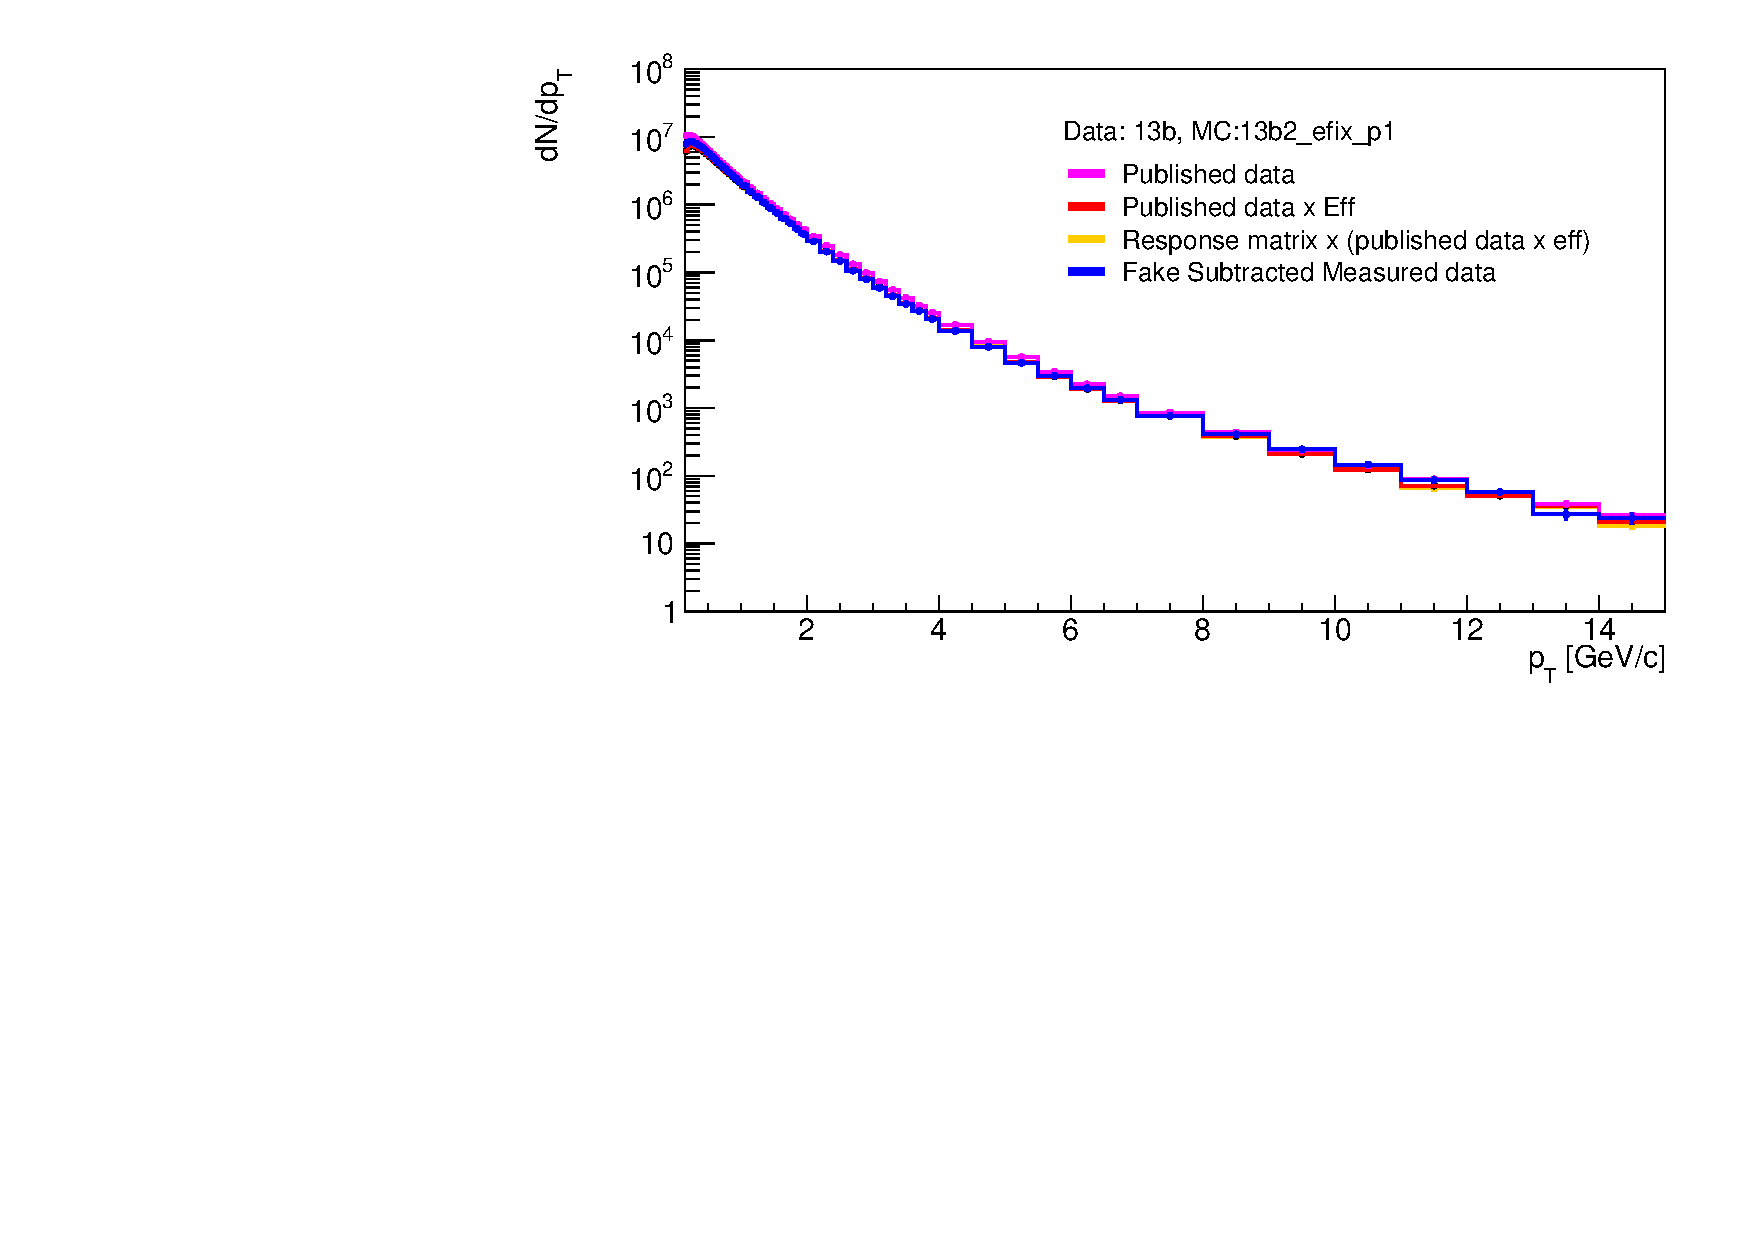
\includegraphics[width=.95\textwidth]{Data_Analysis/Tracking/refolding_pPb_tpc_MBMC_0GeV15GeV_dNdpt.pdf}
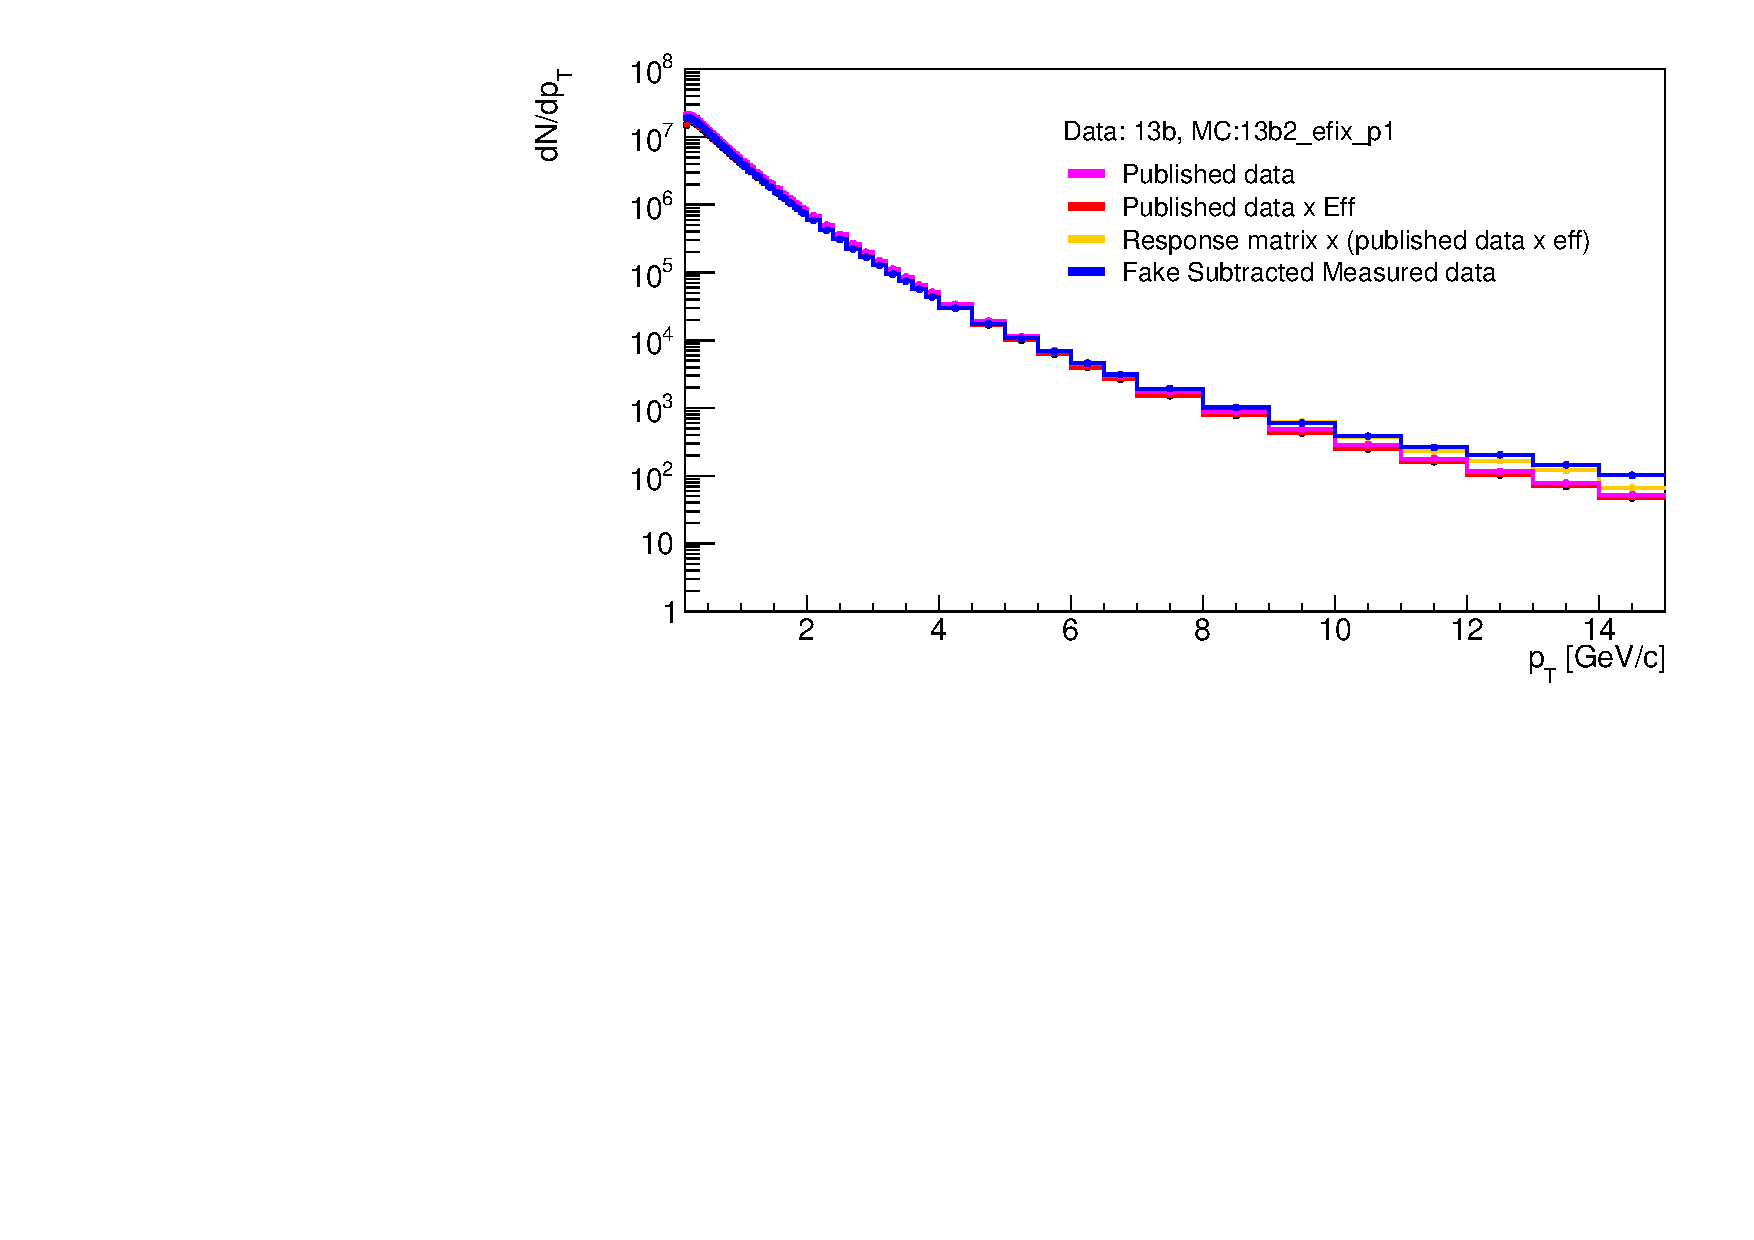
\includegraphics[width=.95\textwidth]{Data_Analysis/Tracking/refolding_pPb_its_MBMC_0GeV15GeV_dNdpt.pdf}
\caption{Smearing of published data at various stages, using TPC+ITS (top) and ITS only (bottom) response matrices. The pink is the published data \pt~spectrum. The red is after the pink has been multiplied by the efficiency. The orange is the spectra after applying the response matrix in order to induce the smearing on the red. The blue is fake-rate-subtracted measured data.}
\label{fig:RefoldedComparisonSpectra}
\end{figure}

The published data has a total uncertainty (quadrature sum of statistical and systematic uncertainties) that ranges from $1.8\%$ at 1 \GeVc, reaches $4.8\%$ by 10 \GeVc~and grows quickly to about 20$\%$ at 15 \GeVc, where it is dominated by the statistical uncertainty. 

Figure~\ref{fig:RefoldedComparison} shows the ratio of the measured fake-subtracted spectrum and the smeared published spectra. The ratio of the published data to the smeared published data is shown to illustrate the impact of the momentum smearing, which is less than a $2\%$ effect for TPC+ITS tracks but it reaches up to a factor of two in the ITS-only case. The closure-test ratios from TPC+ITS tracking are consistent with unity within uncertainties, which is expected. The more interesting result is that the ratios due to ITS-only tracking are within $\pm$5\% of unity in the range between 0.85--10 \GeVc and within $\pm$8\% of unity in the range between 0.5--0.85 \GeVc, shown by the dashed lines in the bottom plot of Figure~\ref{fig:RefoldedComparison}, which is the range we use for our $\gammaiso$--hadron analysis. We will be using this difference from unity as our systematic uncertainty on the tracking.

\begin{figure}[h!]
\center
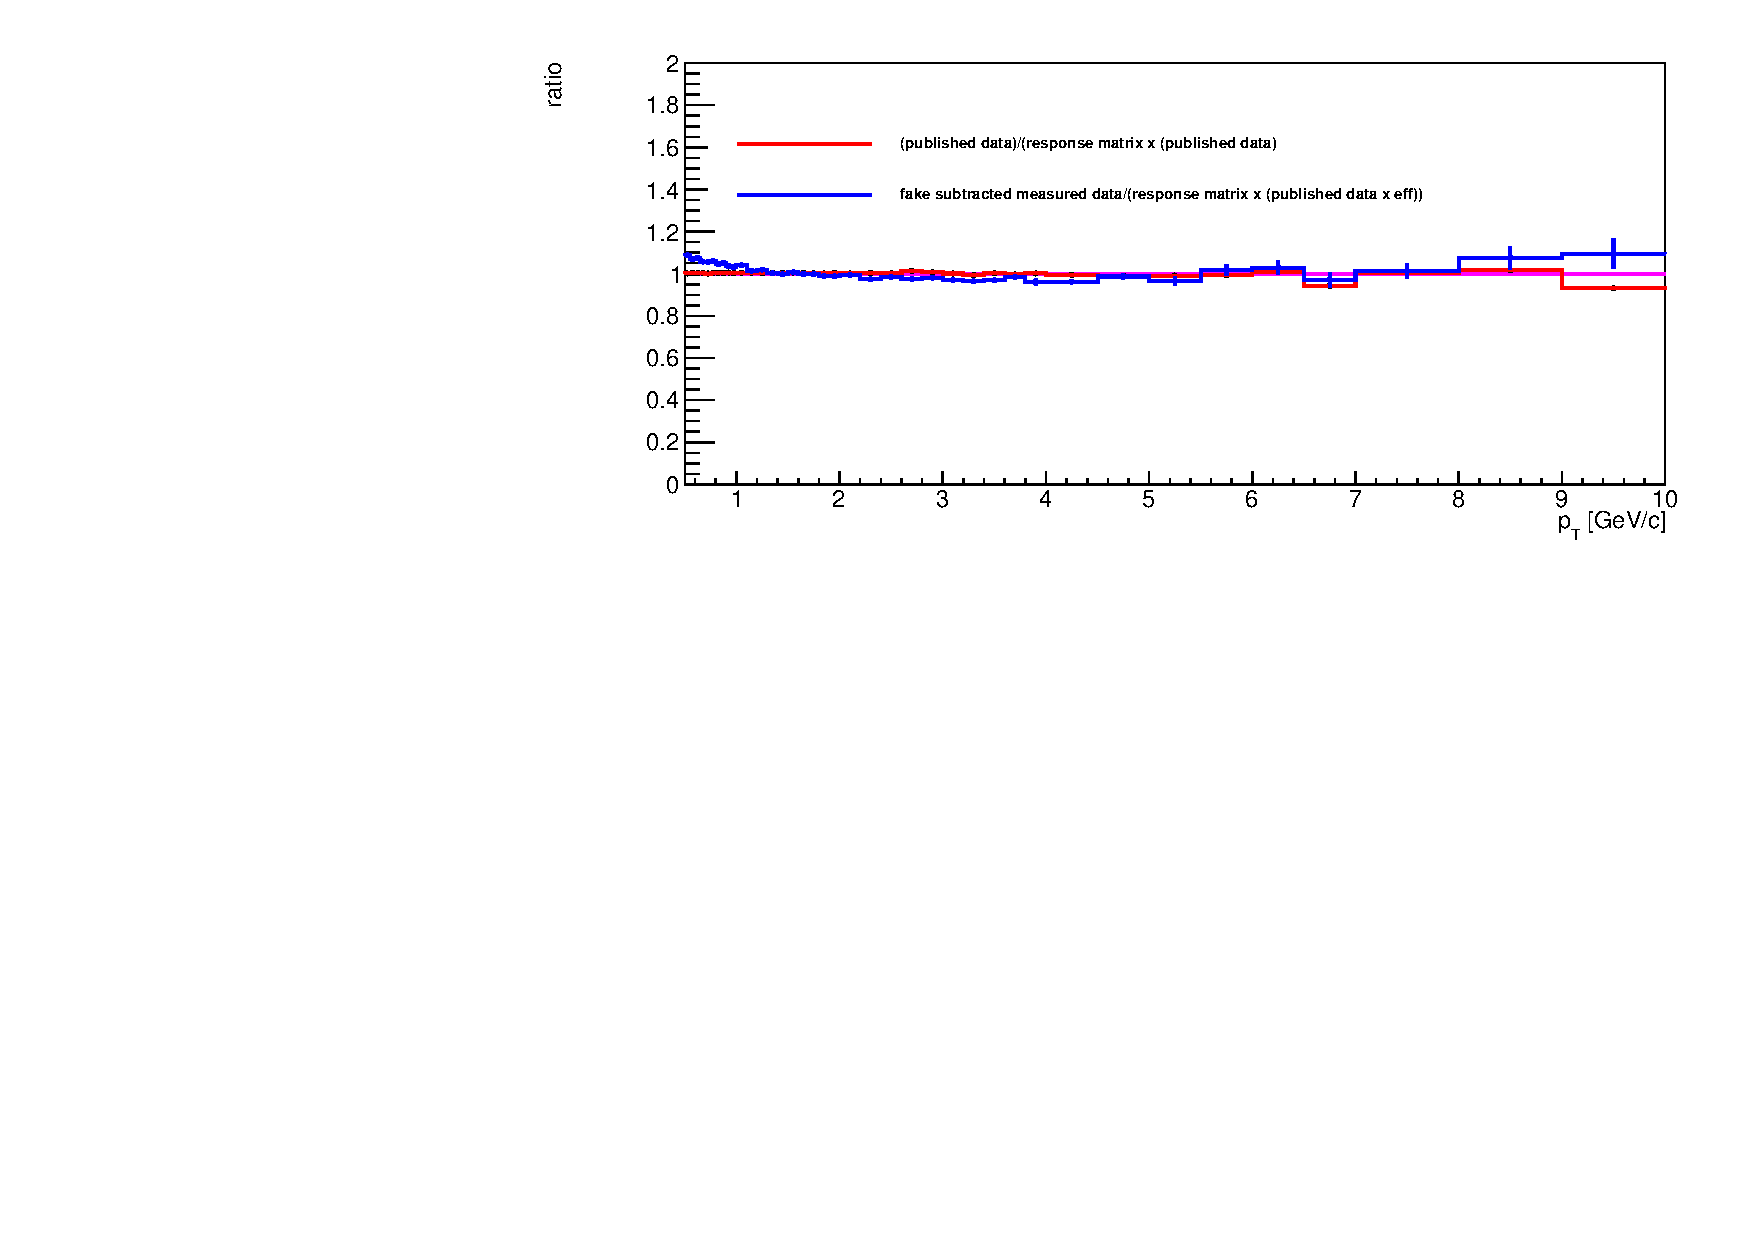
\includegraphics[width=.95\textwidth]{Data_Analysis/Tracking/ratio_refolding_pPb_tpc_MBMC_1GeV15GeV_errors.pdf}
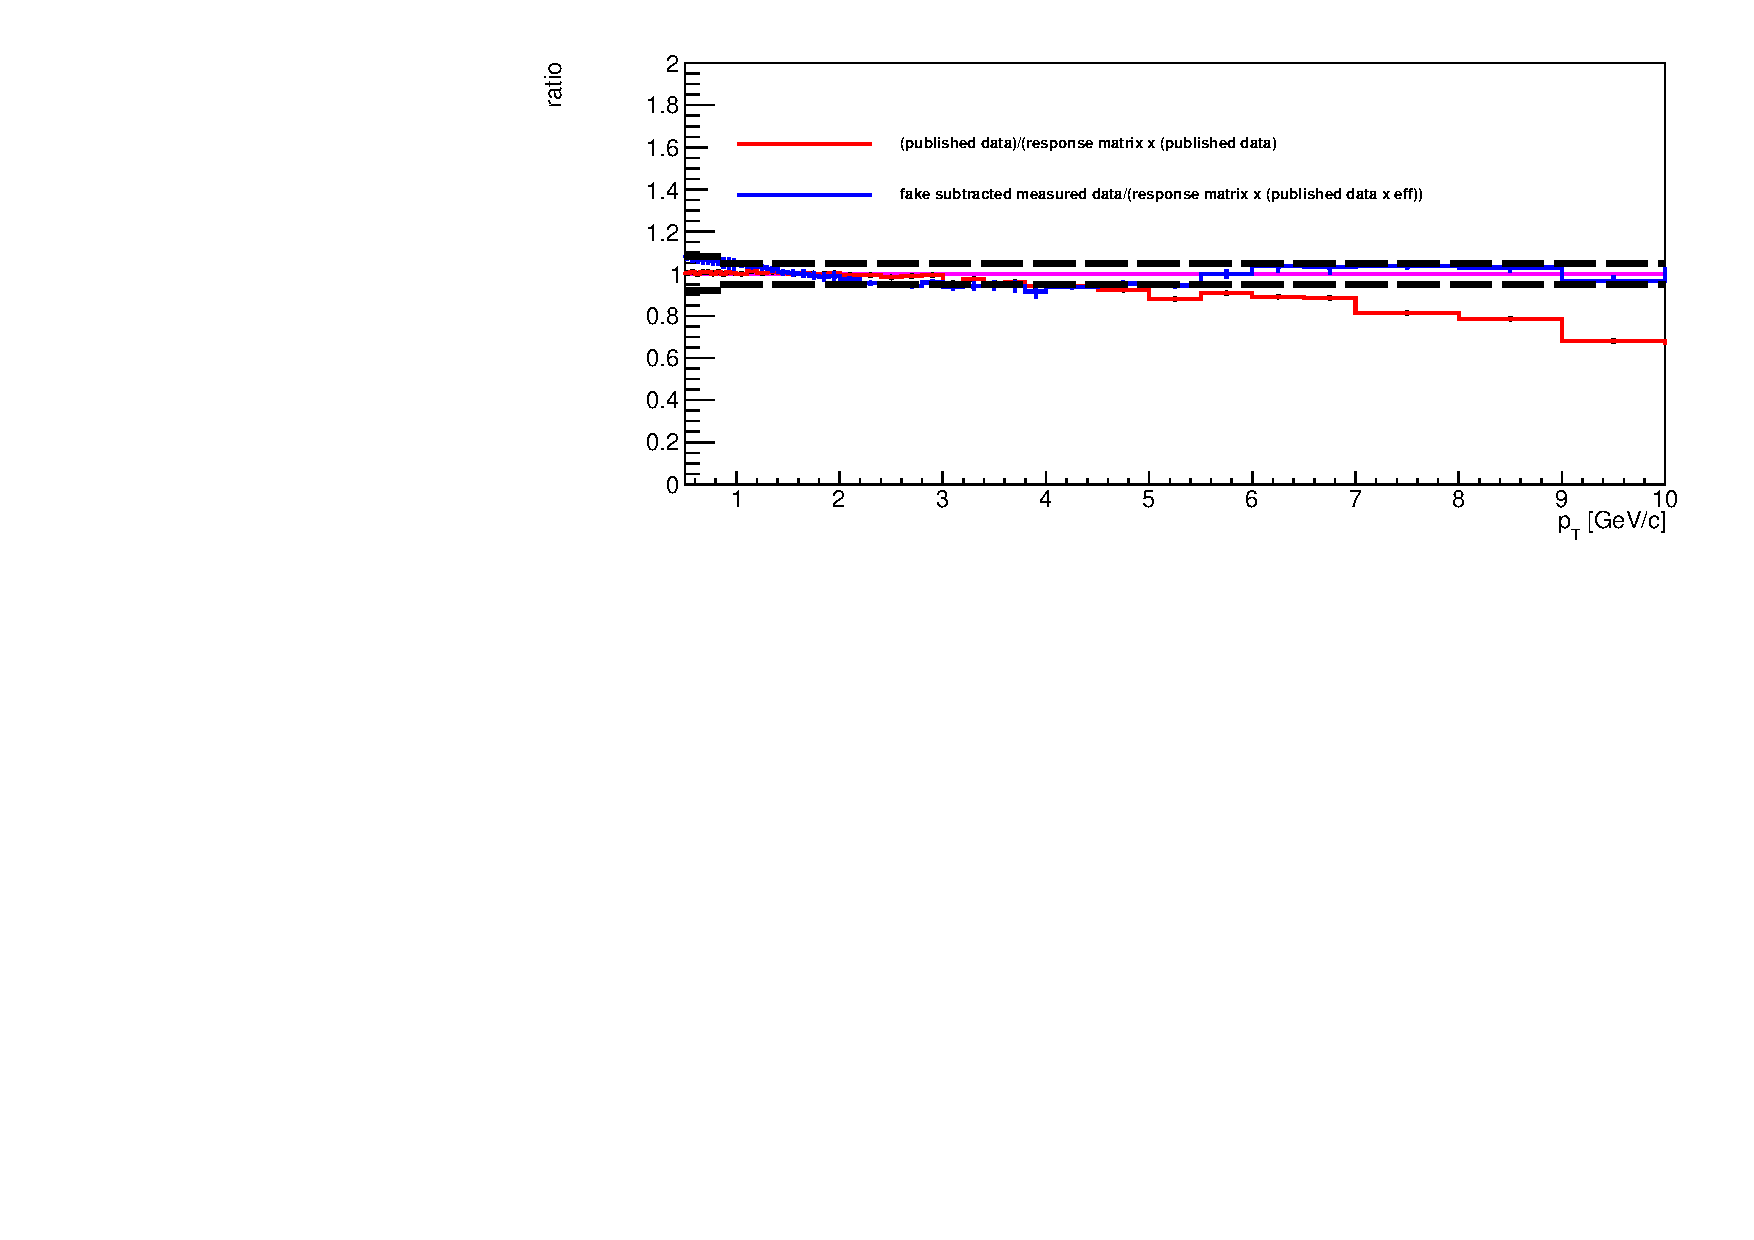
\includegraphics[width=.95\textwidth]{Data_Analysis/Tracking/ratio_refolding_pPb_its_MBMC_0GeV15GeV_errors_band.pdf}
\caption{Result of closure test comparing measured data and published data, for TPC+ITS tracking (top) and ITS-only tracking (bottom). The red curves show the ratio of the reference spectra to the smeared reference spectra. The blue curves show the ratio of the fake-subtracted measured data and the smeared reference spectra. Ideally the blue curve would be flat at unity. The error bar represents statistical uncertainty only for the blue curve, and the quadrature sum of statistical and systematic uncertainties for the red curve. Additionally, the dashed lines from 0.5 to 0.85 \GeVc represent an 8\% band around 1, while the dashed lines from 0.85 to 10.0 \GeVc represent a 5\% band around 1.}
\label{fig:RefoldedComparison}
\end{figure}

The statistically-significant deviation from the published data with ITS-only tracking at high $\pt$ (blue curve in lower panel of Figure~\ref{fig:RefoldedComparison}), could be due to several reasons  including improper modeling of a rapid deterioration of the momentum resolution and underestimation of fake rate. Further work would be needed to understand and correct these and other effects at high $\pt$, but that lies beyond the scope of this work. 

We note that these spectra are normalized per-minimum bias event and not by integral, so the fact that the ratios are close to unity reflect the fact that the efficiency calculations shown in Figure~\ref{fig:tpcEff} are an accurate description of the detector response. Based on the results shown in this section, we restrict $\pt$ range to no more than 10 \GeVc, which is beyond the limit of the statistical power of our $\gammaiso$-hadron analysis. 
 % and quote $\pm$5$\%$ as a systematic uncertainty for tracking performance for tracks with {0.5 $<\pt<$ 10 \GeVc}. 

\FloatBarrier
\subsubsection{Angular dependence of tracking efficiency}
Here, we demonstrate that the $\varphi$-dependence of holes in the ITS-only tracking is well reproduced in the MC simulation. The 2D $\varphi$-$\eta$ efficiency is calculated in a similar way to the $\pt$ efficiency described in Equation~\ref{eq:eff}, but instead of being functions of $\pt^{\mathrm{true}}$, the efficiency is a function of the true track azimuthal angle and pseudorapidity, $\varphi^{\mathrm{true}}$ and $\eta^{\mathrm{true}}$ respectively. Only tracks with {$\pt^{\mathrm{true}}>1$} \GeVc~are consider to avoid strong effects of bending due to the magnetic field that would obscure the impact of dead regions.

\begin{figure}[h]
\center
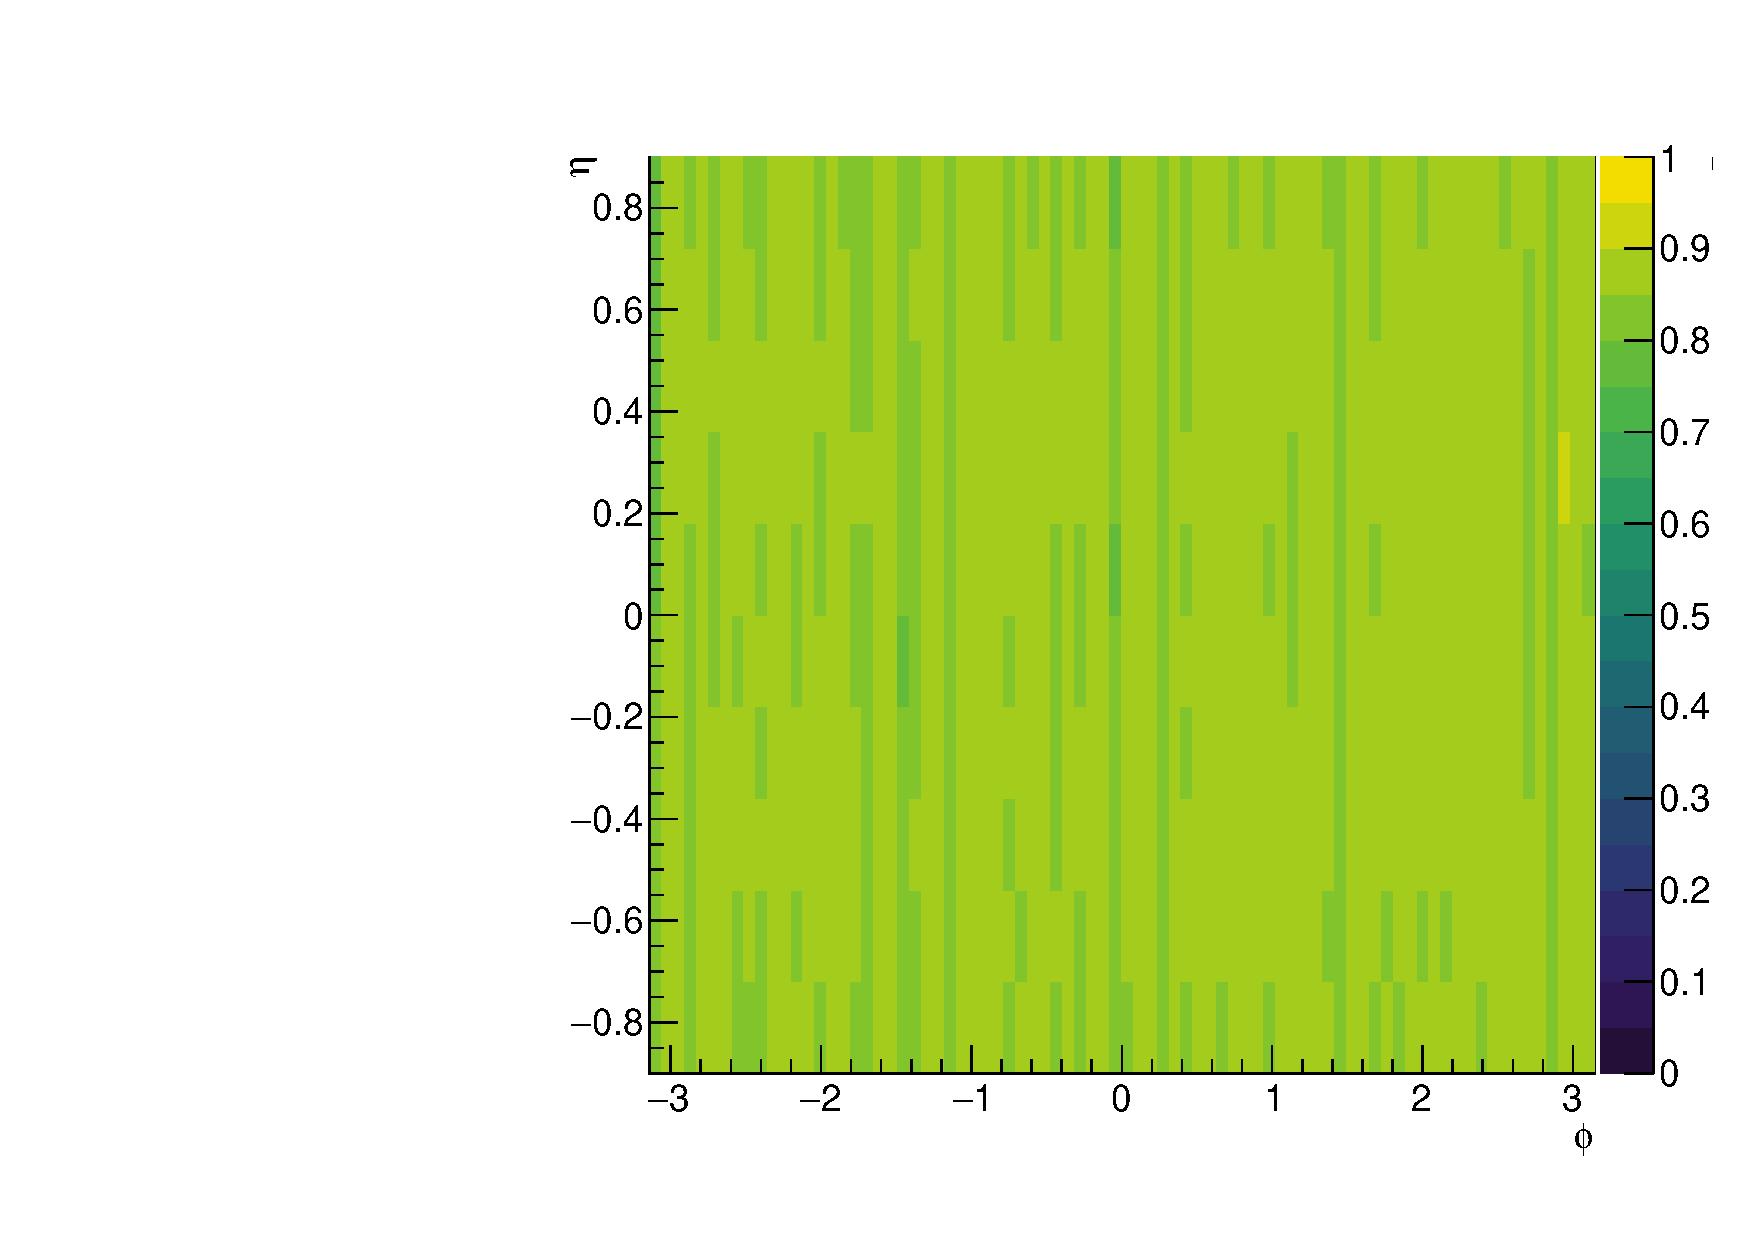
\includegraphics[width=0.46\textwidth]{Data_Analysis/Tracking/etaPhi_eff_tpc.pdf}
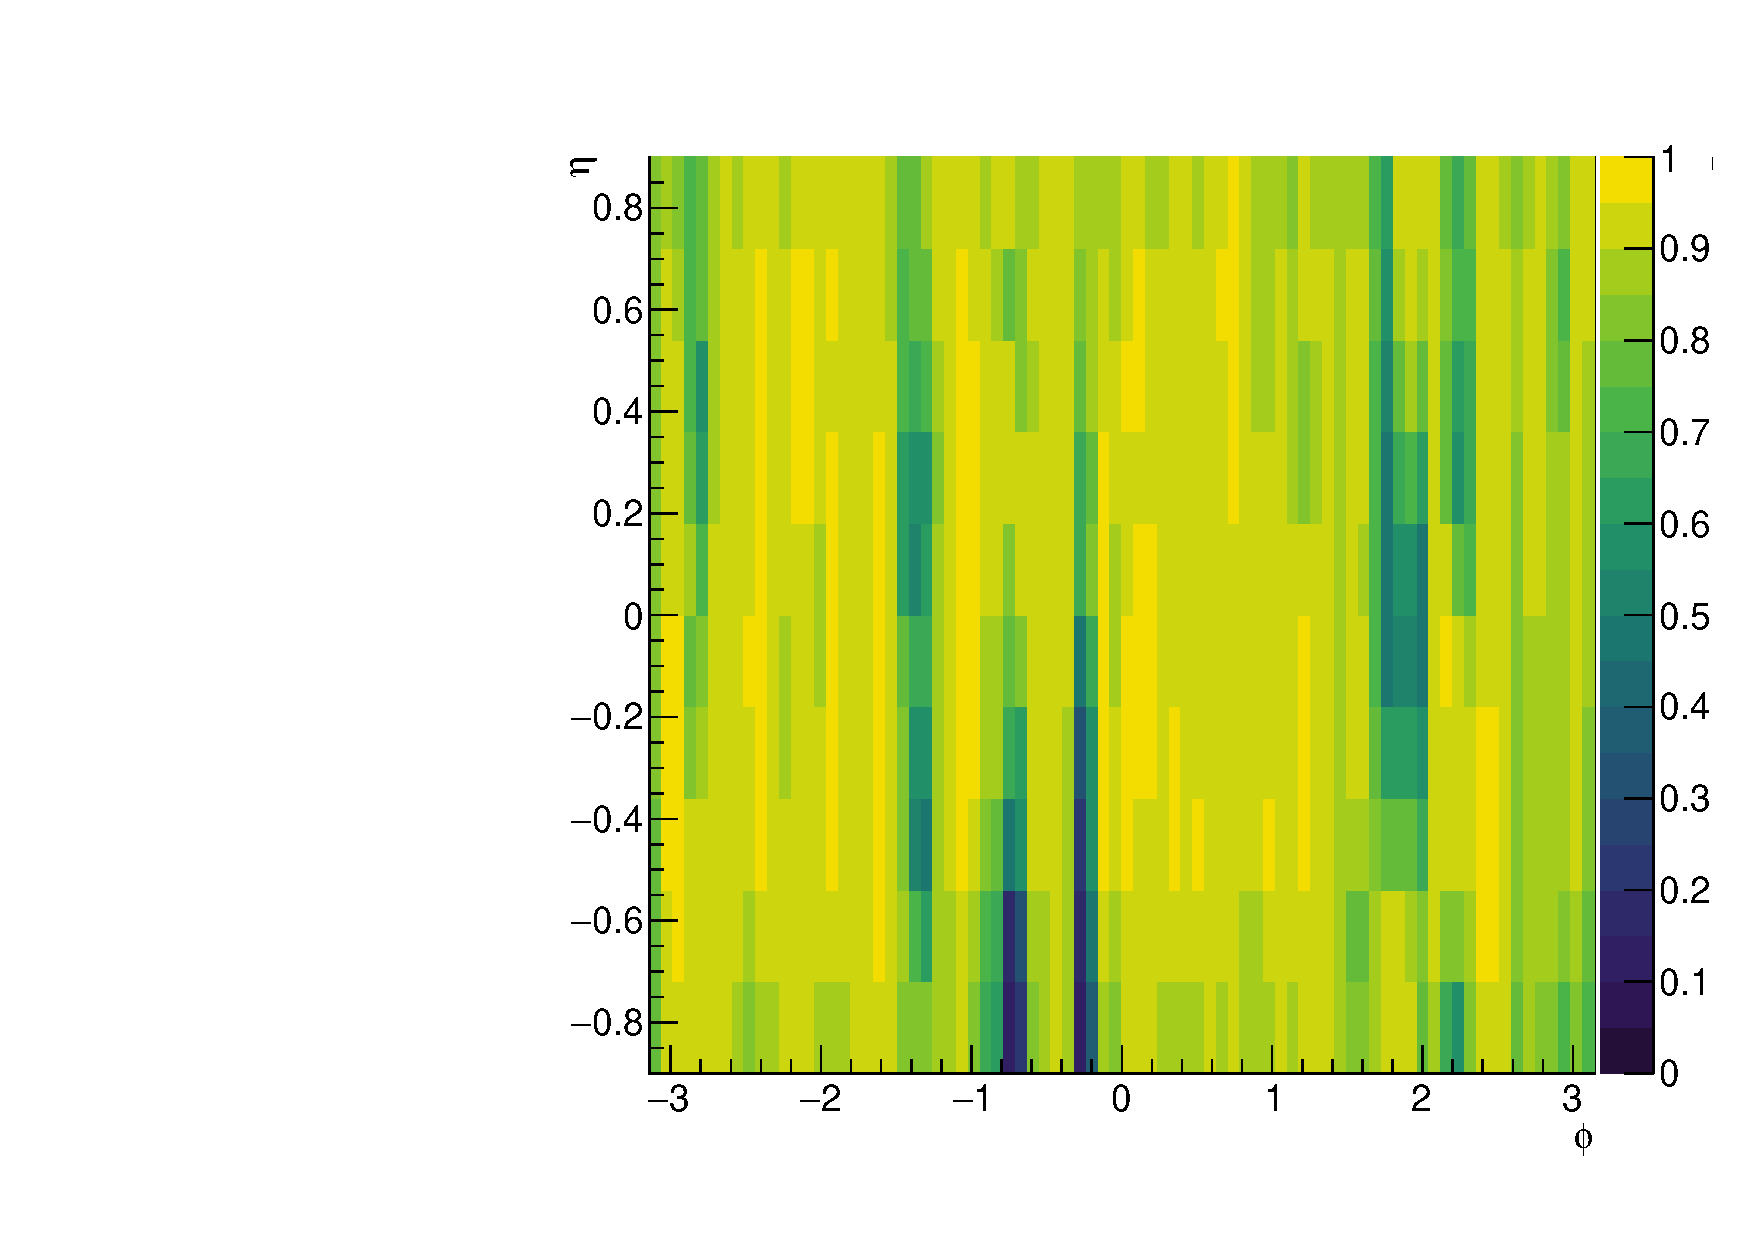
\includegraphics[width=0.46\textwidth]{Data_Analysis/Tracking/etaPhi_eff_4layers.pdf}
\caption{Tracking efficiency as a function of $\varphi^{\mathrm{true}}$ and $\eta^{\mathrm{true}}$ for TPC+ITS (left) and ITS-only (right) tracks.}
\label{fig:2Defficiency}
\end{figure}

Figure~\ref{fig:2Defficiency} shows the resulting efficiency for TPC+ITS and ITS-only tracks. While the TPC+ITS 2D $\varphi$-$\eta$ distribution looks uniform, this is not the case for the ITS-only distribution, which has visible dips in the efficiency at various $\varphi$. The efficiency is close to unity for most of the phase space covered. There are no big $\eta$ variations, but there are large $\varphi$ variations. The efficiency holes at $\varphi$ = $-$0.8 and $-$0.2 are very visible and reach values close to zero. These are attributed to ITS-staves that are completely dead. Any variations in $\varphi$ in the $\gammaiso$-hadron analysis are corrected for using the event mixing technique described in Section \ref{sec:EventMixing}

\subsubsection{Validation of $\varphi$-dependence of efficiency}
\label{sec:phicheck}

In order to validate the description of the ITS-only tracking holes, we do a test with minimum-bias data. For this, we rely on the fact that apart from the effect of $\varphi$-dependent holes, the track azimuthal angle distribution is expected to be uniform in minimum-bias data. So we measure the track $\varphi$ spectrum, then correct for the efficiency and check whether the distribution is flat. The level of flatness gives us a sense of the systematic uncertainties associated with mis-modeling of the $\varphi$-dependent efficiency.

Figure~\ref{fig:phiEff} shows the $\varphi$-dependence of the tracking efficiency for TPC+ITS and ITS-only tracks. The efficiency is calculated using Equation~\ref{eq:eff}, but as a function of $\varphi^{true}$ instead of \pt~$^{true}$. The TPC+ITS tracking efficiency is flat in $\varphi$ as expected, but there are dips in the efficiency for the ITS-only tracking due to dead staves in the ITS. These have little impact on the TPC+ITS tracks because the selection does not have the strict requirement on the number of ITS hits, $N_{\mathrm{ITS}} \geq$ 4, that is applied for ITS-only tracks. 

\begin{figure}[h]
\center
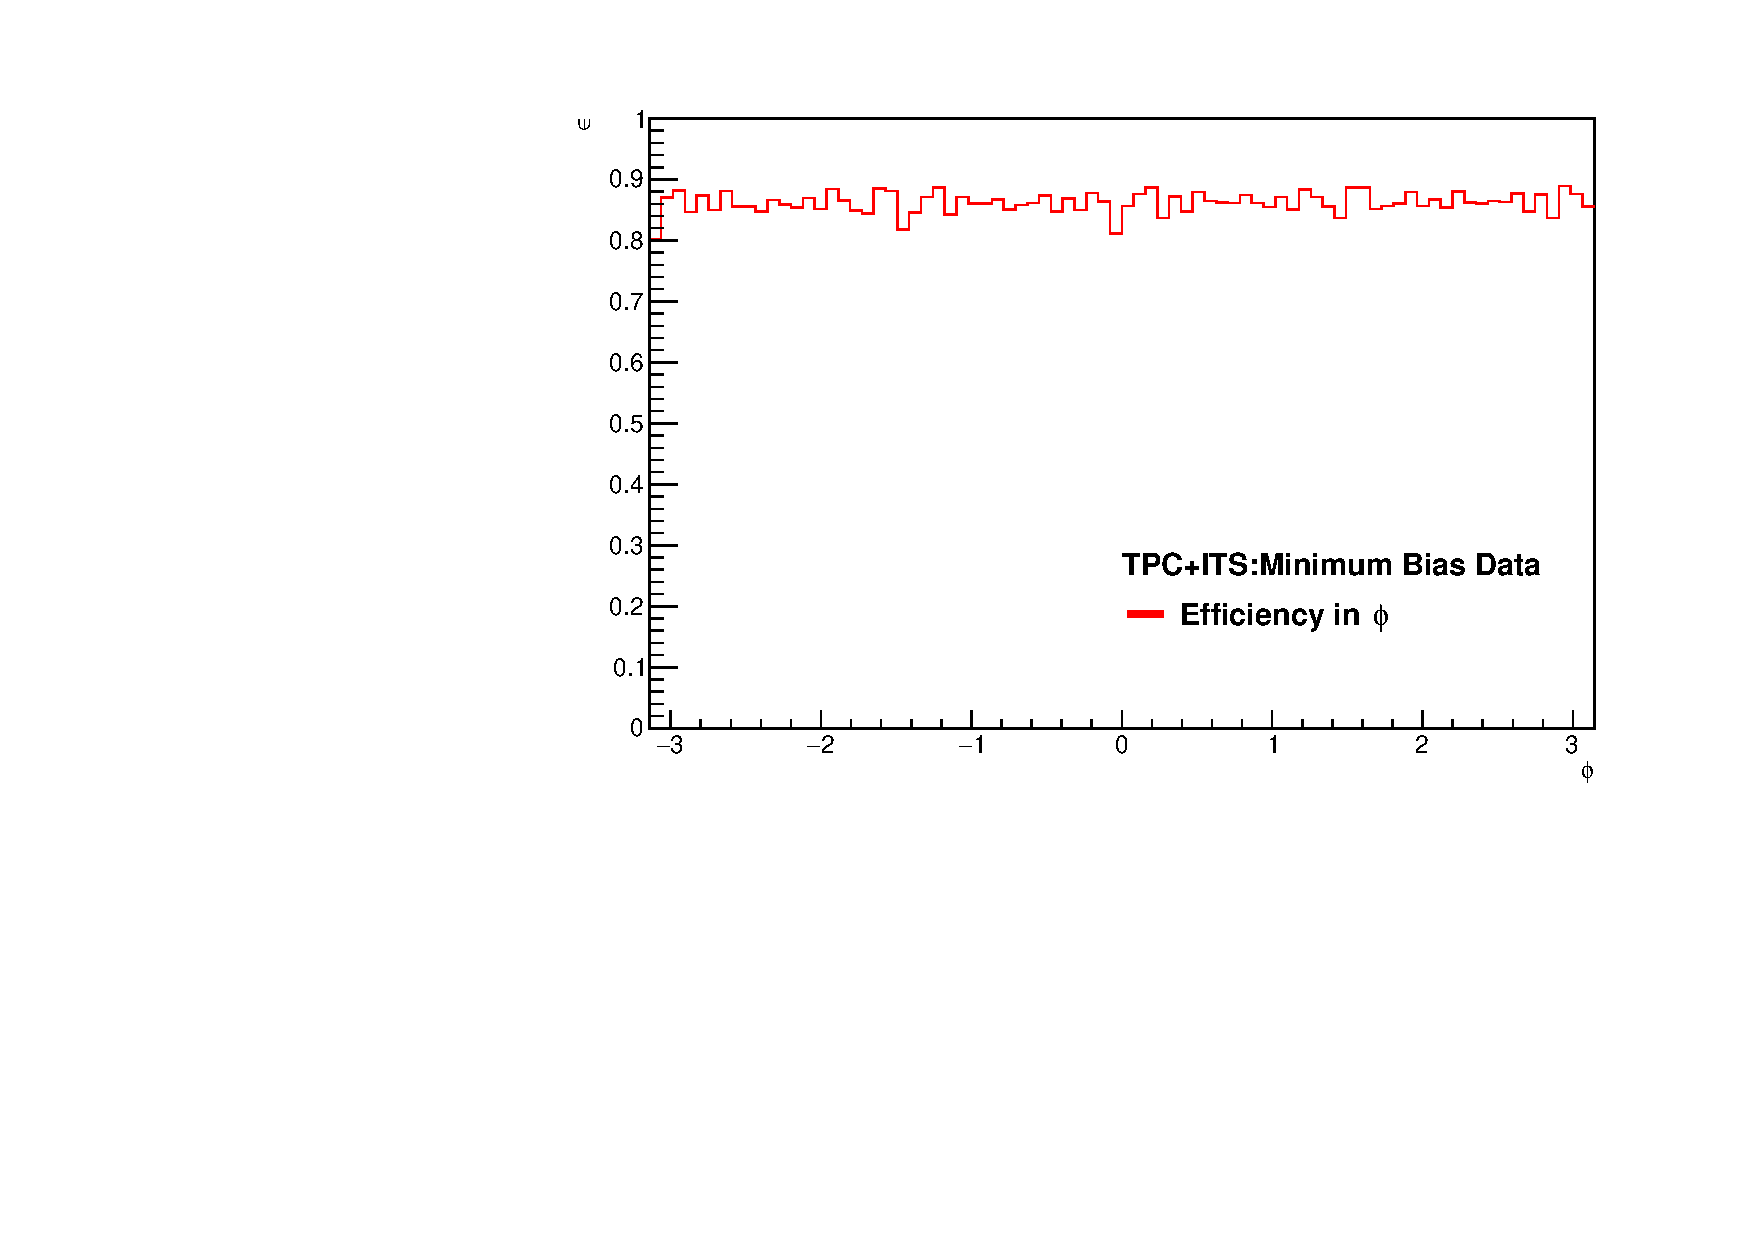
\includegraphics[width=.495\textwidth]{Data_Analysis/Tracking/tpc_phi_eff.pdf}
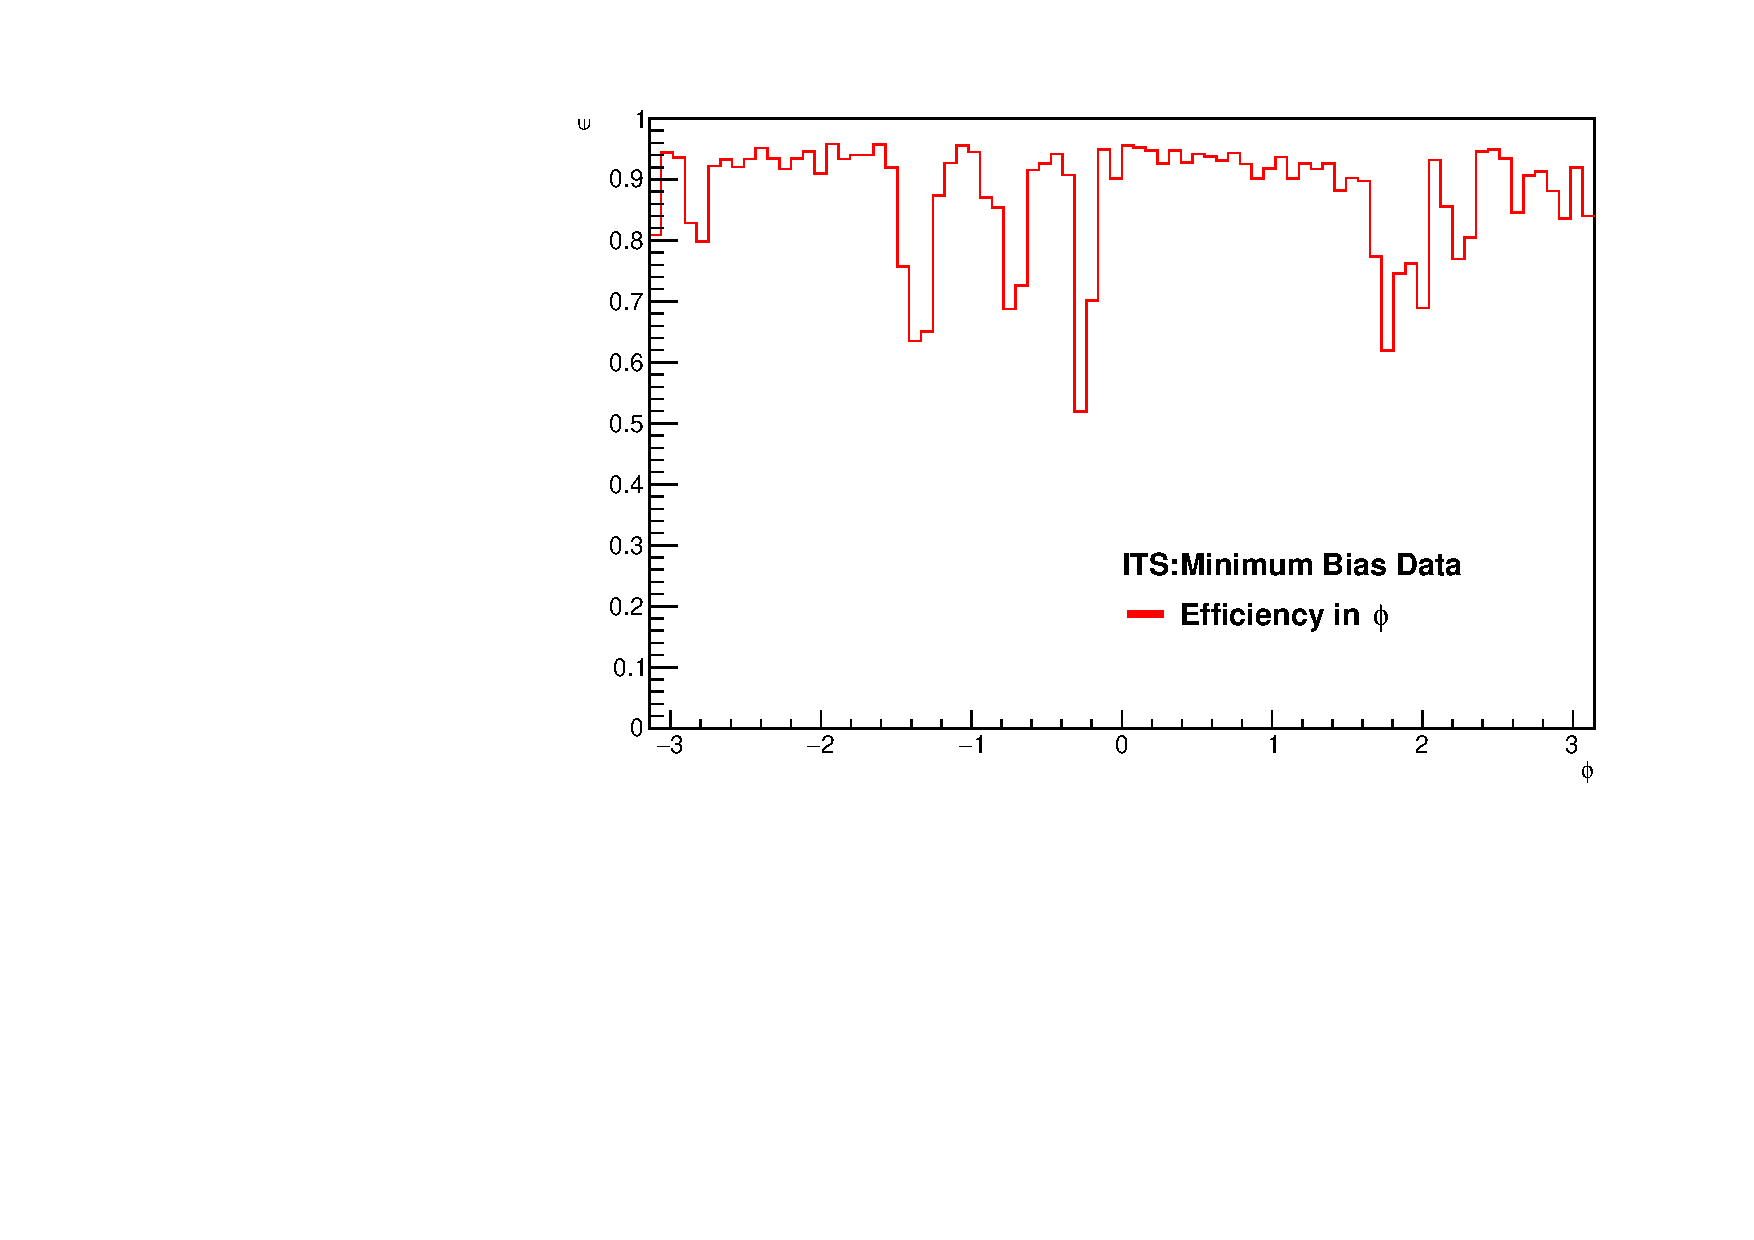
\includegraphics[width=.495\textwidth]{Data_Analysis/Tracking/its_phi_eff.pdf}
\caption{Tracking efficiency as a function of $\phi^{\mathrm{true}}$ for TPC+ITS tracks (left) and ITS-only tracks (right). In both cases, the efficiency is calculated for tracks with $\pt^{\mathrm{true}}>$ 1 \GeVc~using the LHC13b2\_efix\_p1 Monte Carlo simulation.}
\label{fig:phiEff}
\end{figure}

\begin{figure}[h]
\center
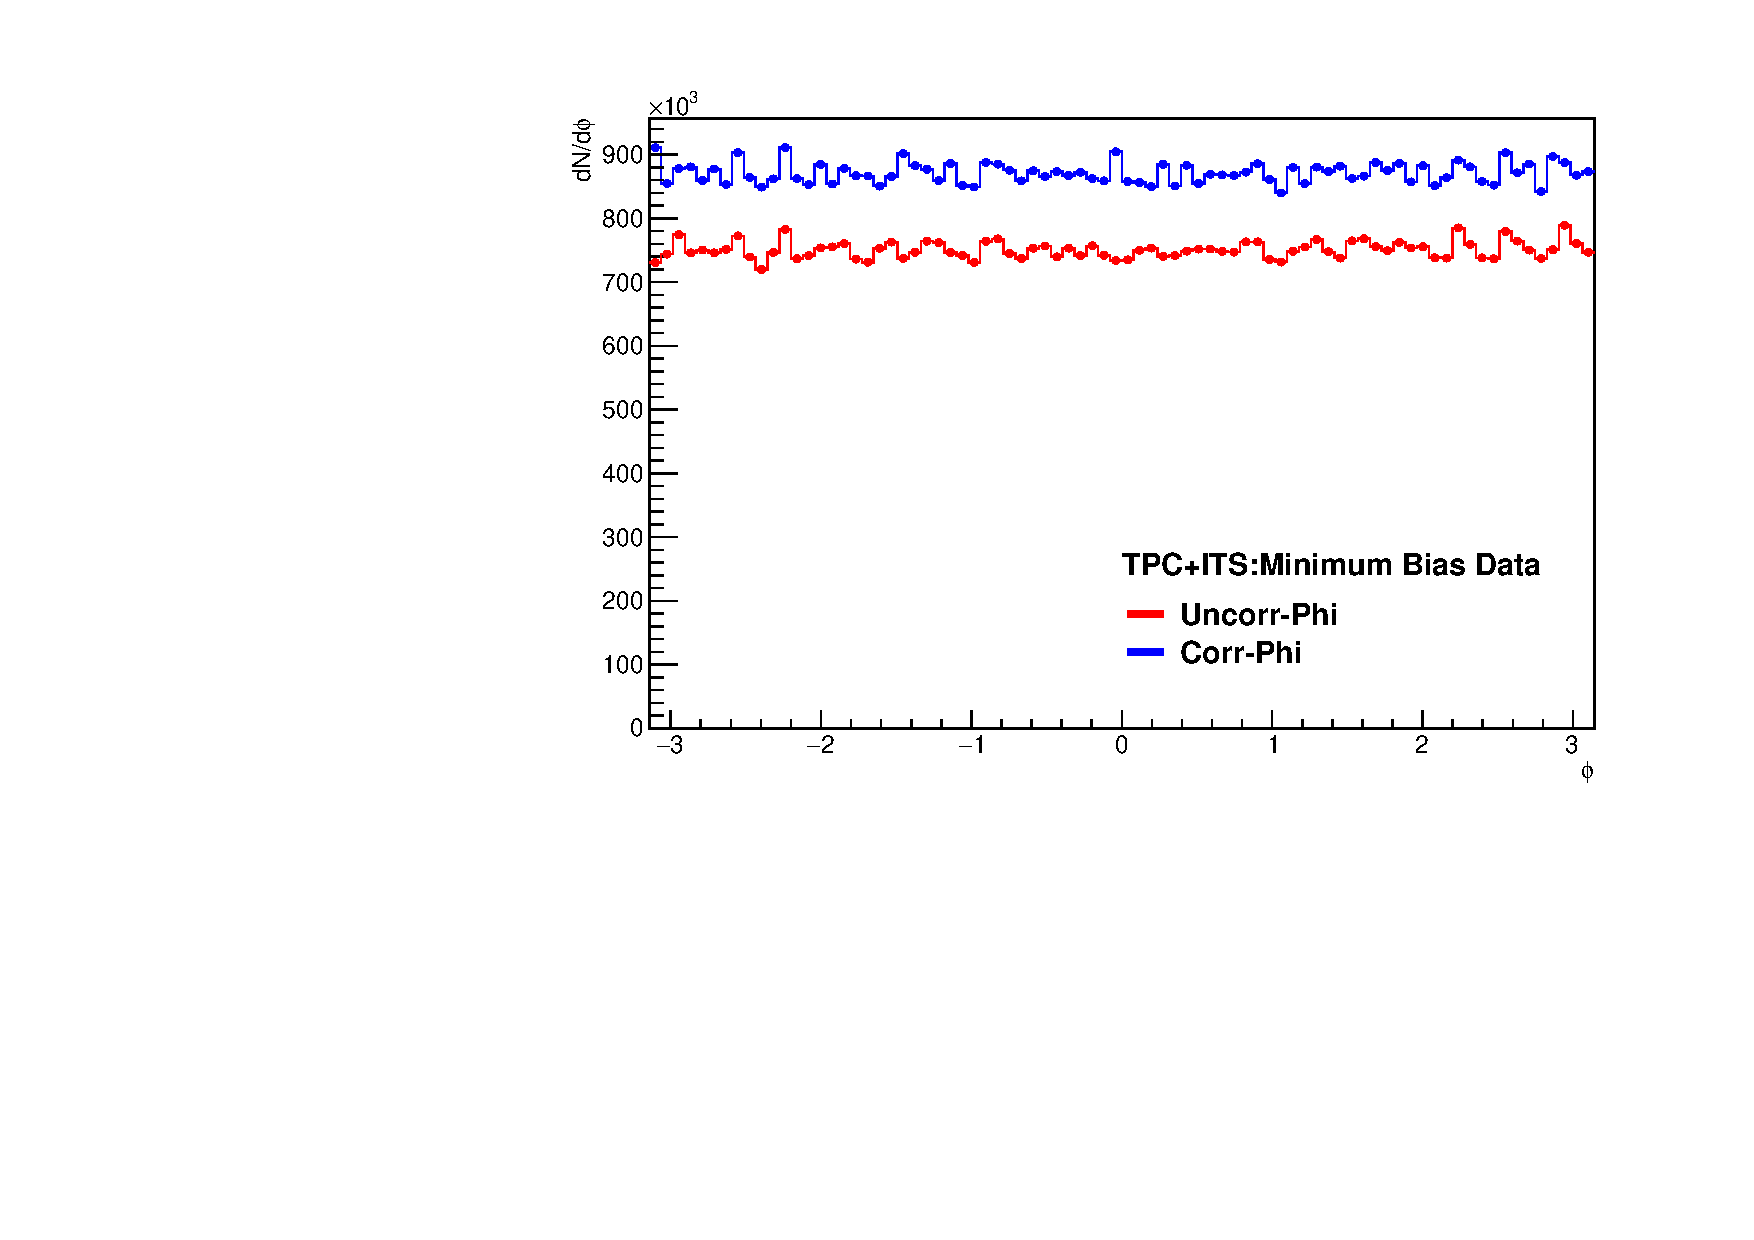
\includegraphics[width=.495\textwidth]{Data_Analysis/Tracking/phi_efficiency_cor_tpc.pdf}
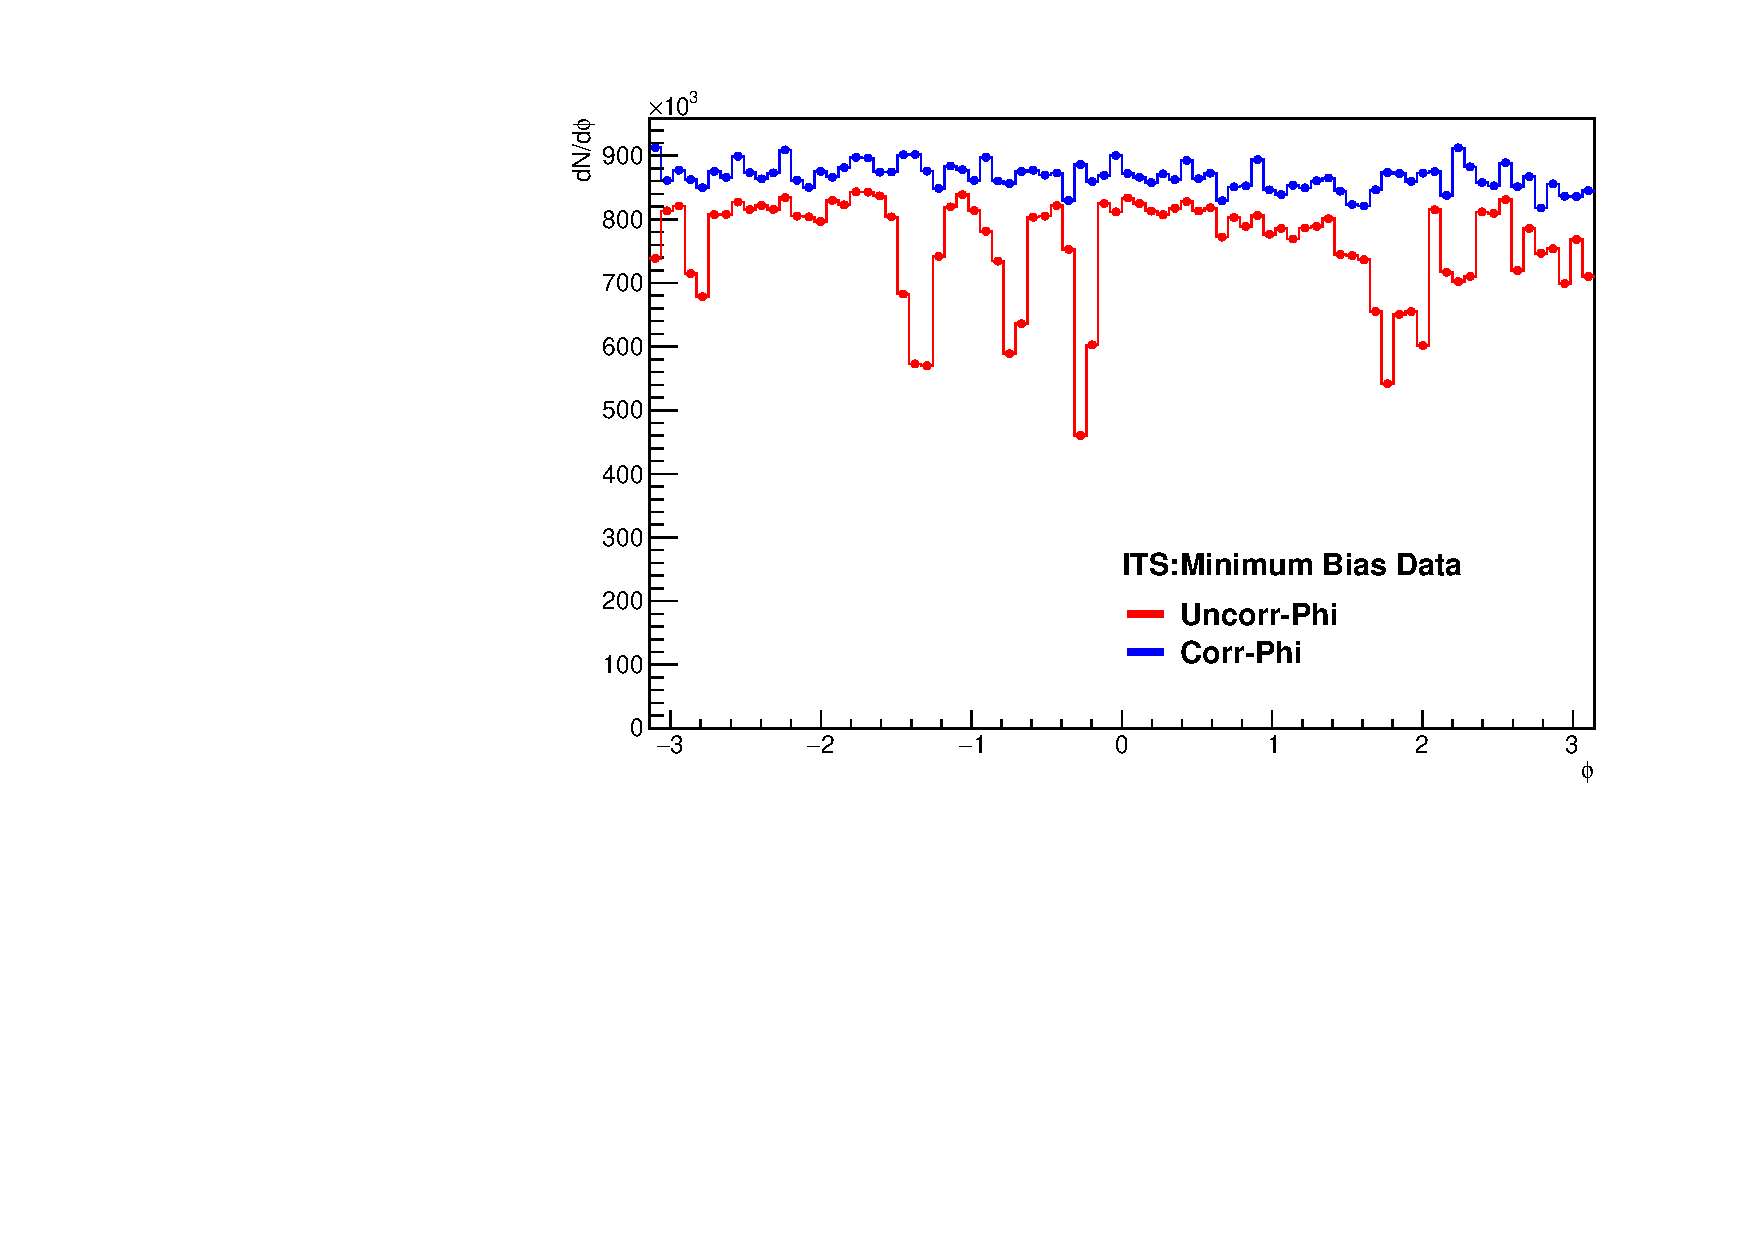
\includegraphics[width=.495\textwidth]{Data_Analysis/Tracking/phi_efficiency_cor_its.pdf}
\caption{Left panel: track $\varphi$ distribution measured in data for tracks with $|\eta|<0.8$ before (red) and after (blue) applying the efficiency correction for TPC+ITS tracks. Right panel:track $\varphi$ distribution measured in data for tracks with $|\eta|<0.8$ before (red) and after (blue) applying the efficiency correction for ITS-only tracks.}
\label{fig:phiCorr}
\end{figure}

Figure~\ref{fig:phiCorr} shows the $\varphi$ distribution of TPC+ITS and ITS-only tracks in minimum-bias \pPb~data and the effect of applying the efficiency correction to the $\varphi$ distribution. Before applying the efficiency correction, there are visible holes at $\varphi$ = $-$1.04, $-$0.8, $-$0.2 rad in ITS-only tracks which are not present in the TPC+ITS tracking. After applying the $\varphi$ efficiency, the holes are corrected, and we obtain a distribution which is flat within {$\pm$2.5\%}. The TPC+ITS remains flat after the efficiency correction, as expected. This shows that the description of dead channels in the ITS is well-described in the simulation. 

\FloatBarrier
\subsection{Summary of the ITS-only tracking performance studies} 
In this section we summarize the findings of our studies on ITS-only tracking performance: 
\begin{enumerate}
\item Tracking Efficiency: \\
The ITS-only tracking efficiency is $75\%$ at 150 MeV/$c$ and grows to 85$\%$ at 1 \GeVc~and above. 
\item Fake rate:\\
The fake rate of ITS-only tracking is about 10 times worse than for TPC+ITS tracks, but still less than 20$\%$ below 10 \GeVc, which is the relevant range for the analyses presented in this note.
\item Momentum resolution:\\
The momentum smearing effects are significant for ITS-only tracking. The bin-to-bin correction factor due to smearing effects for ITS-only tracking is 0.7 at 10~\GeVc~and 0.5 at 15~\GeVc. The smearing effects for ITS+TPC tracking are negligible.
\item Description of $\varphi$ holes\\
The efficiency as a function of $\varphi$ shows inhomogeneity not present in the TPC+ITS tracking that are attributed to dead staves in the ITS. These are concentrated in specific $\eta$ and $\varphi$ regions. These are well described in the simulation. 
\end{enumerate}

We have validated the MC corrections for tracking efficiency, fake rate and momentum smearing by comparing with published data. From that study, we estimate a combined systematic uncertainty on tracking performance to be a relative $\pm 5\%$ for ITS-only tracks with $0.5 < \pt < 10$ \GeVc. 

%\FloatBarrier
%\subsubsection{Fake Rate Subtraction}
%The fake rate is negligible in TPC+ITS but significant in the ITS-only tracking, especially at high $\pt$. The number of fakes for each $\pt$ is determined by taking the product of the measured data and the fake rate in that $\pt$ interval. Then, the number of fakes is subtracted from the number of tracks in the measured data to obtain the fake-subtracted spectrum, as shown in Figure~\ref{fig:fksub}. Due to a larger fake rate at high $\pt$ in ITS-only tracking, we can see a deviation from the measured spectrum at high $p_T$.
%\begin{figure}[h]
%\center
%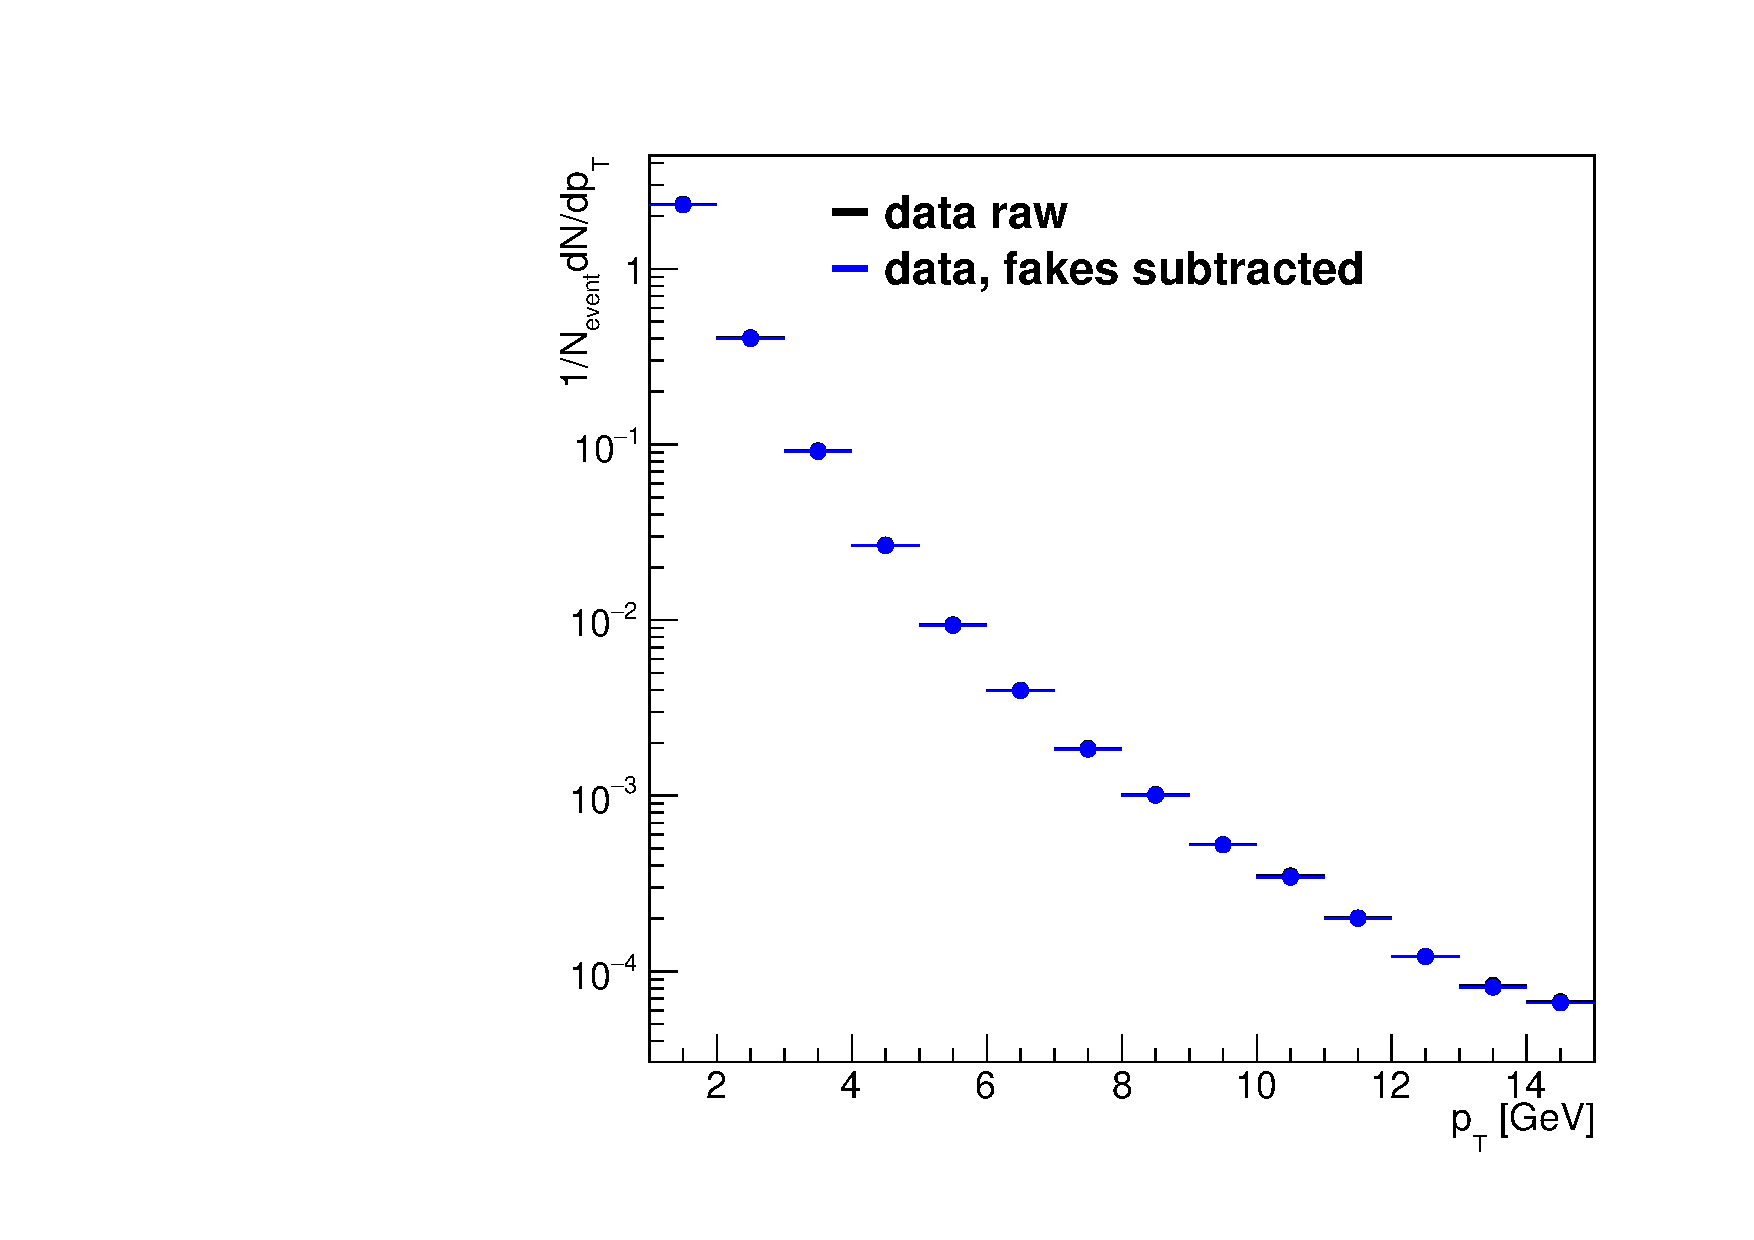
\includegraphics[width=.49\textwidth]{Data_Analysis/Tracking/FakeRate_sub_tracking_tpc_MBMC_1GeV15GeV.pdf}
%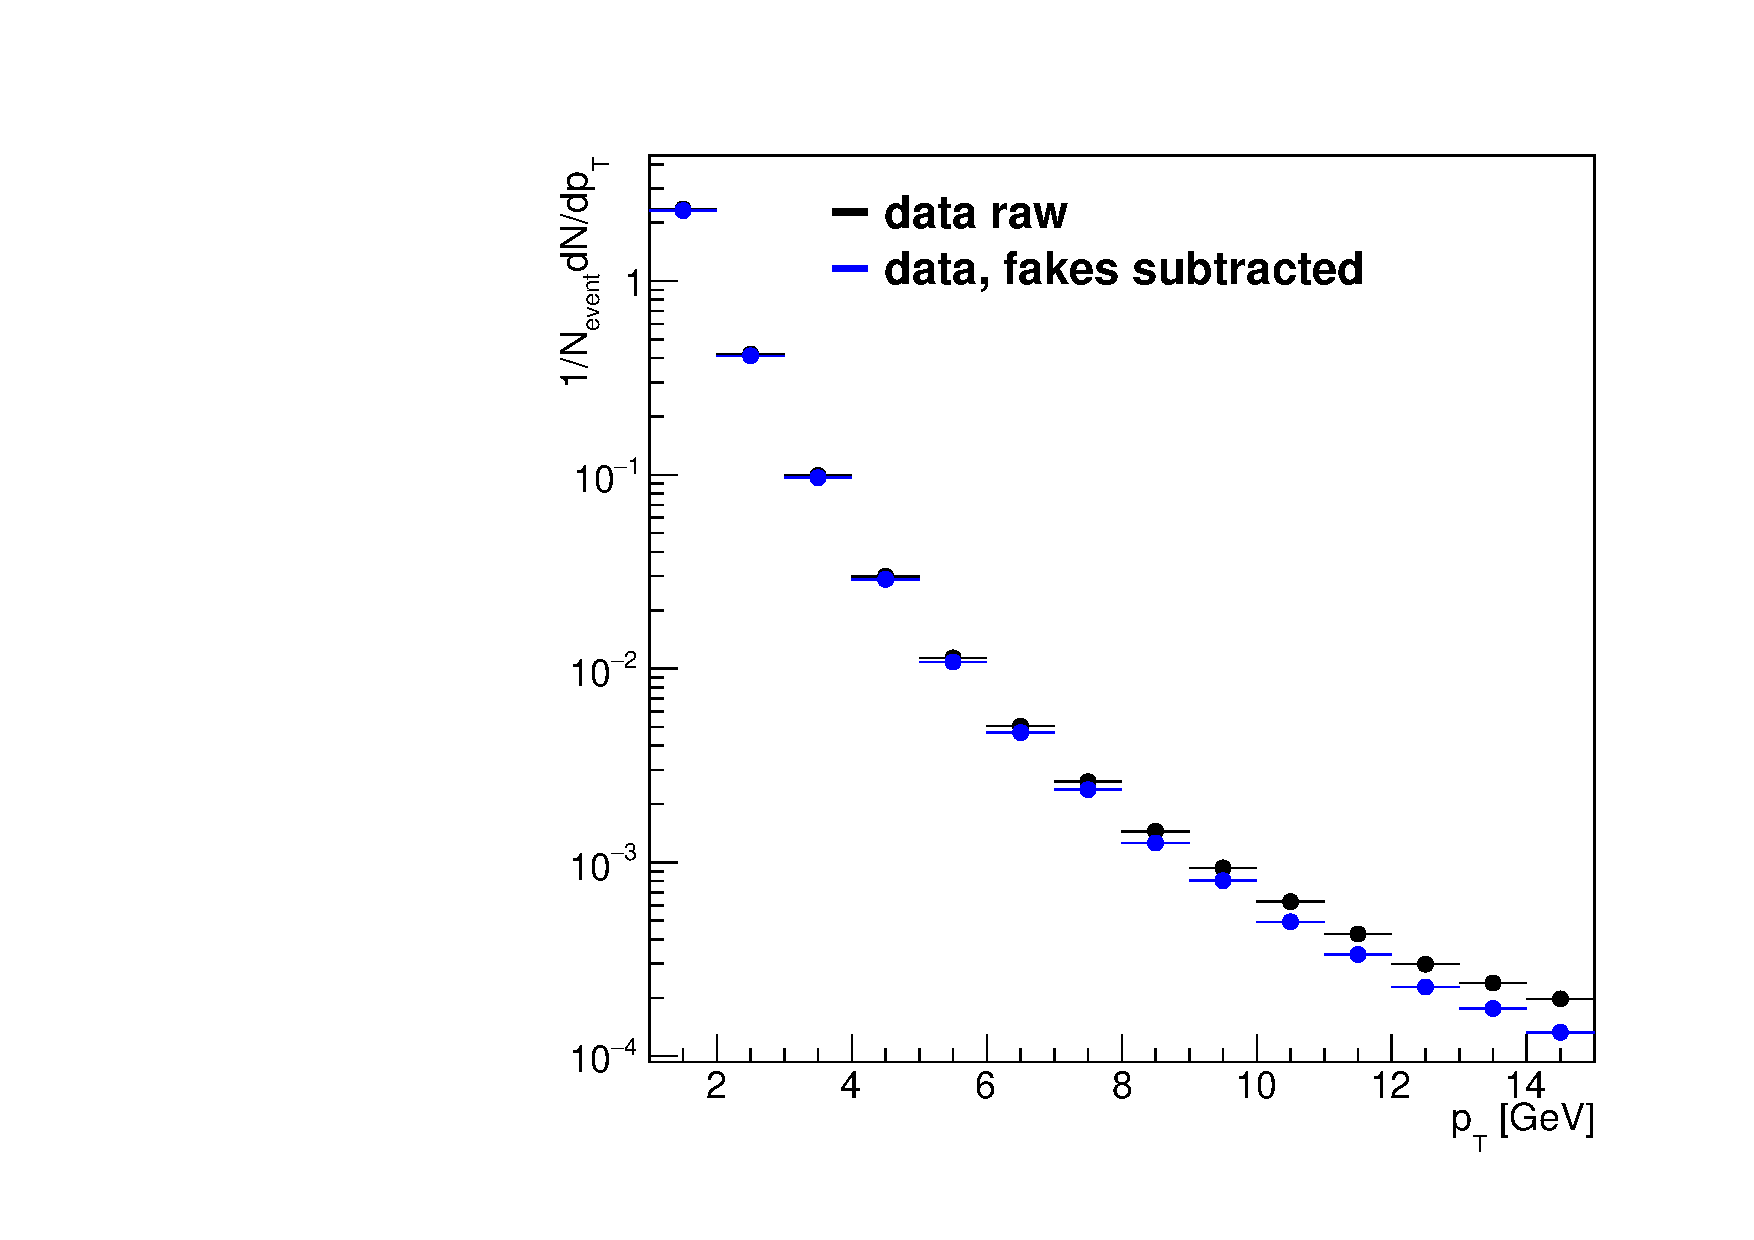
\includegraphics[width=.49\textwidth]{Data_Analysis/Tracking/FakeRate_sub_tracking_its_MBMC_1GeV15GeV.pdf}
%\caption{A comparison between TPC+ITS (left) and ITS-only(right) of the measured spectrum (data, raw) and the measured spectrum after subtracting the fakes (data, fakes subtracted). The statistical uncertainty of the data is typically smaller than the marker size.}
%\label{fig:fksub}
%\end{figure}
%\subsubsection{Smearing}
%Removed, not PC for TPC-lovers. 
%What we have shown is an unprecedented result in ALICE. For comparison, previous results using ITS-only tracks have been restricted to $\pt<$ 1 \GeVc. This measurement establishes a benchmark for tracking performance that opens up an opportunity to measure hard-probes at a high rate (i.e, without TPC) during Run-3 with the new bigger, better and faster ITS, and at the high-luminosity LHC.  
%igure~\ref{fig:etaEff} shows the efficiency with respect to the $\eta$ of the tracks. The efficiency is calculated using equation~\ref{eq:eff}, but as a function of $\eta^{true}$, instead of $\pt^{true}$. %The efficiency in the $\eta$ direction is flat. While figure~\ref{fig:etaEff} shows the $\eta$ efficiency for all tracks with $\pt > 1 \GeVc$, figure~\ref{fig:etaEff_diffpt} shows the $\eta$ efficiency for selected \pt ranges between $0.15 \GeVc - 2.0 \GeVc$. As we can see the 


%\begin{figure}[h]
%\centering
%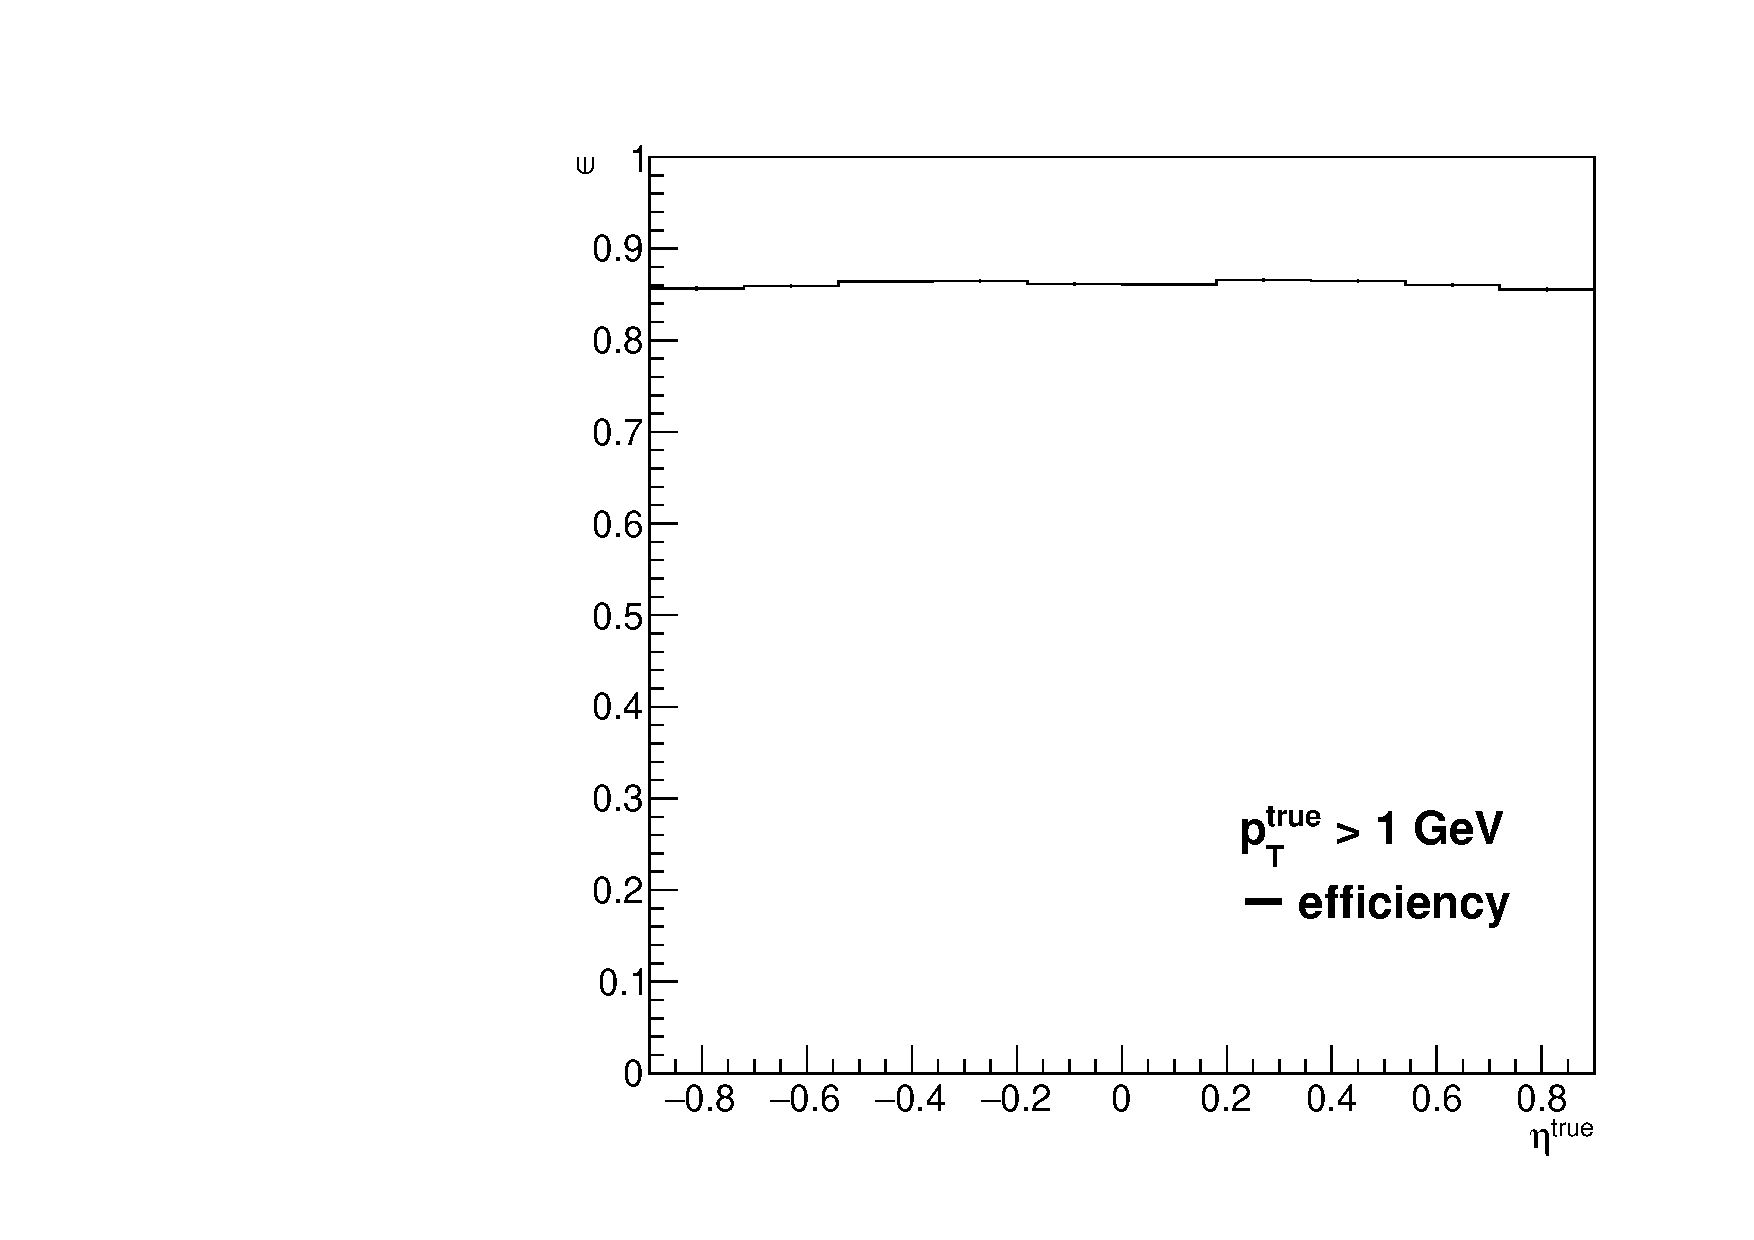
\includegraphics[width=.49\textwidth]{Data_Analysis/Tracking/its_eta_eff.pdf}
%\caption{The efficiency of the $\eta$ variable of the tracks using the LHC13b2\_efix\_p1 Monte Carlo simulation}
%\label{fig:etaEff}
%\end{figure}

%\begin{figure}[h]
%\centering
%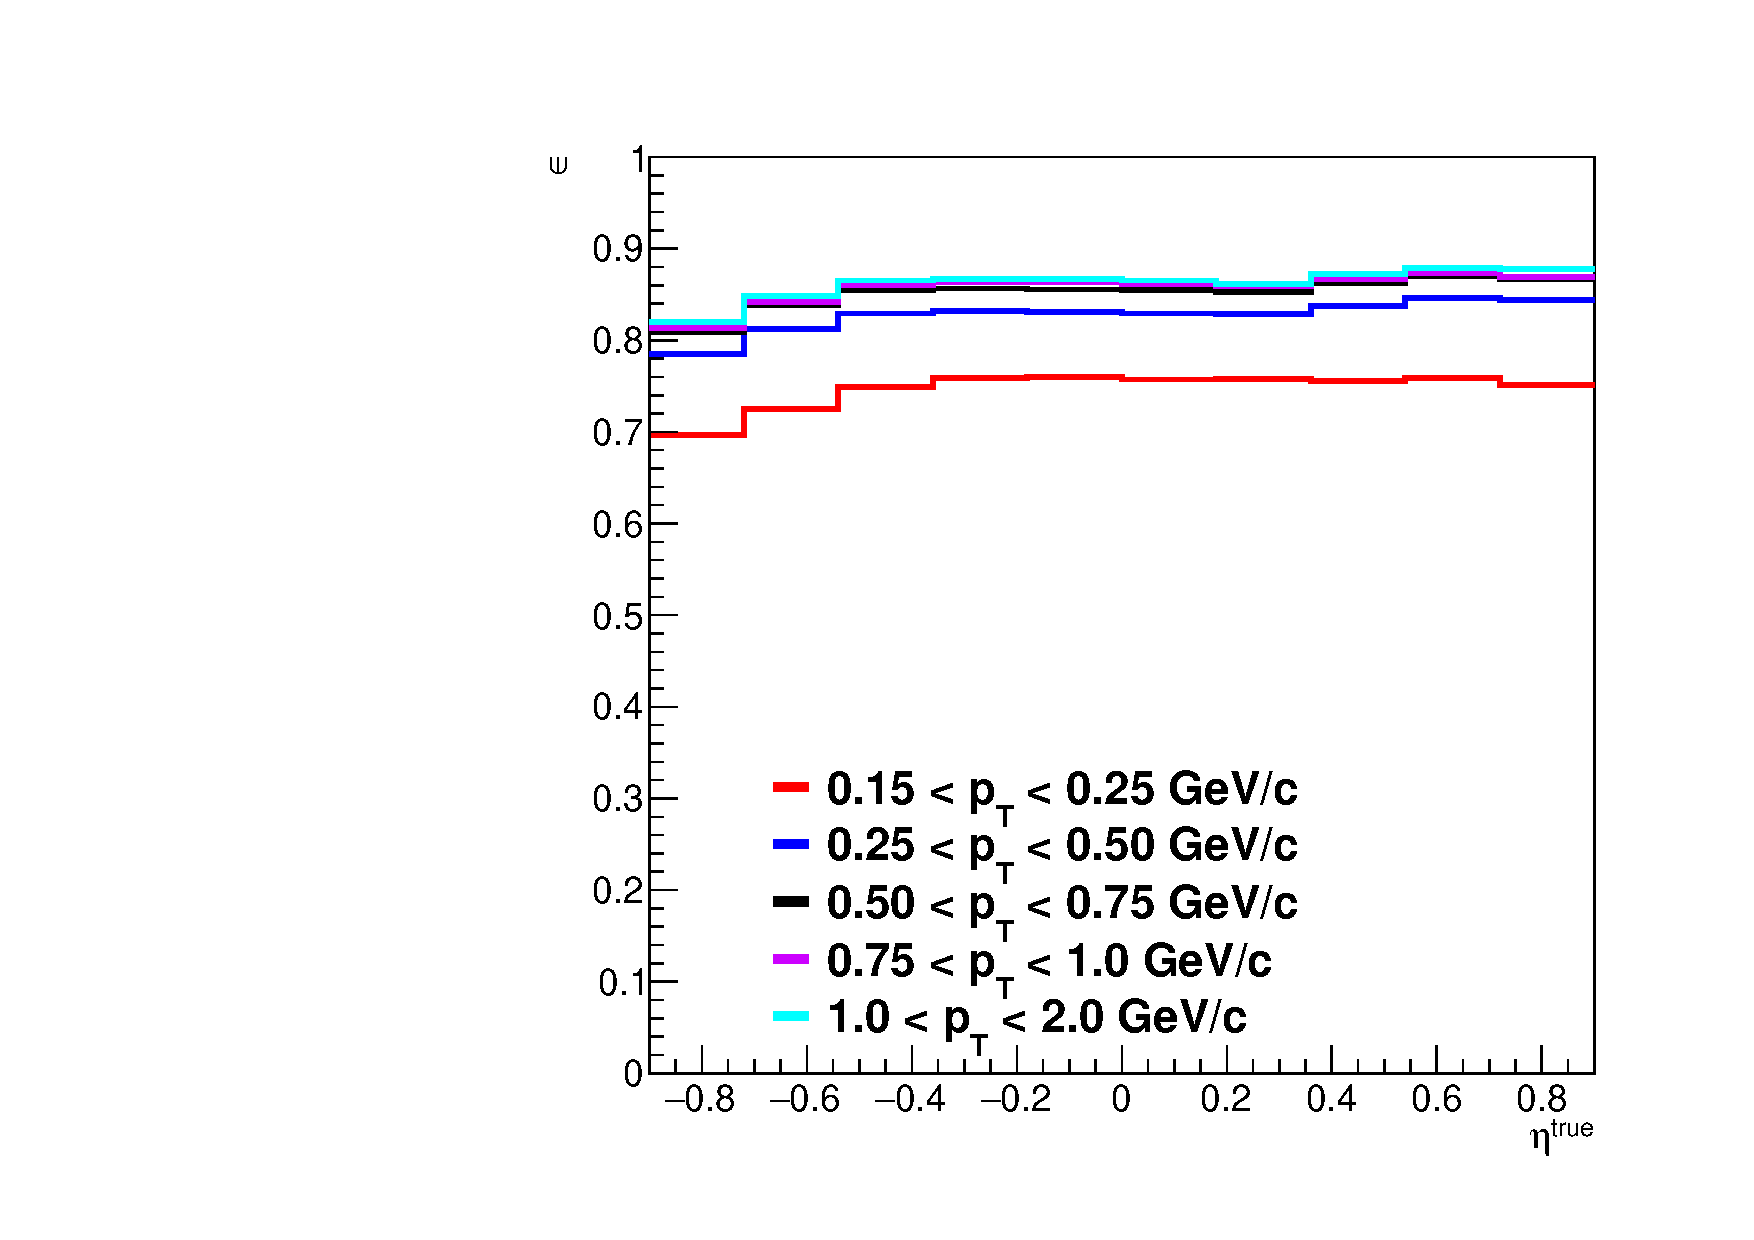
\includegraphics[width=.49\textwidth]{Data_Analysis/Tracking/etaEff_diffpt.pdf}
%\caption{The efficiency of the $\eta$ variable of the tracks for different \pt ranges using the LHC13b2\_efix\_p1 Monte Carlo simulation}
%\label{fig:etaEff_diffpt}

%\end{figure}


%Figure~\ref{fig:gaussian_reso} illustrates the resulting momentum resolution for ITS-only and TPC+ITS tracks for representative momentum ranges. The distributions for ITS-only tracks are significantly wider in both low and high $\pt$ ranges. The relative difference between reconstructed and generated momentum follows roughly a Gaussian shape, but with fatter tails. 

%The high $\pt$ curve for ITS-only tracks is asymmetric at high $\pt$, being significantly biased towards lower-than-true reconstructed values. This is expected as multiple-scattering and other smearing effects would tend to make a straight track less straight, and thus be reconstructed with lower momentum, but not the other way around. 

%\begin{figure}[h]
%\center
%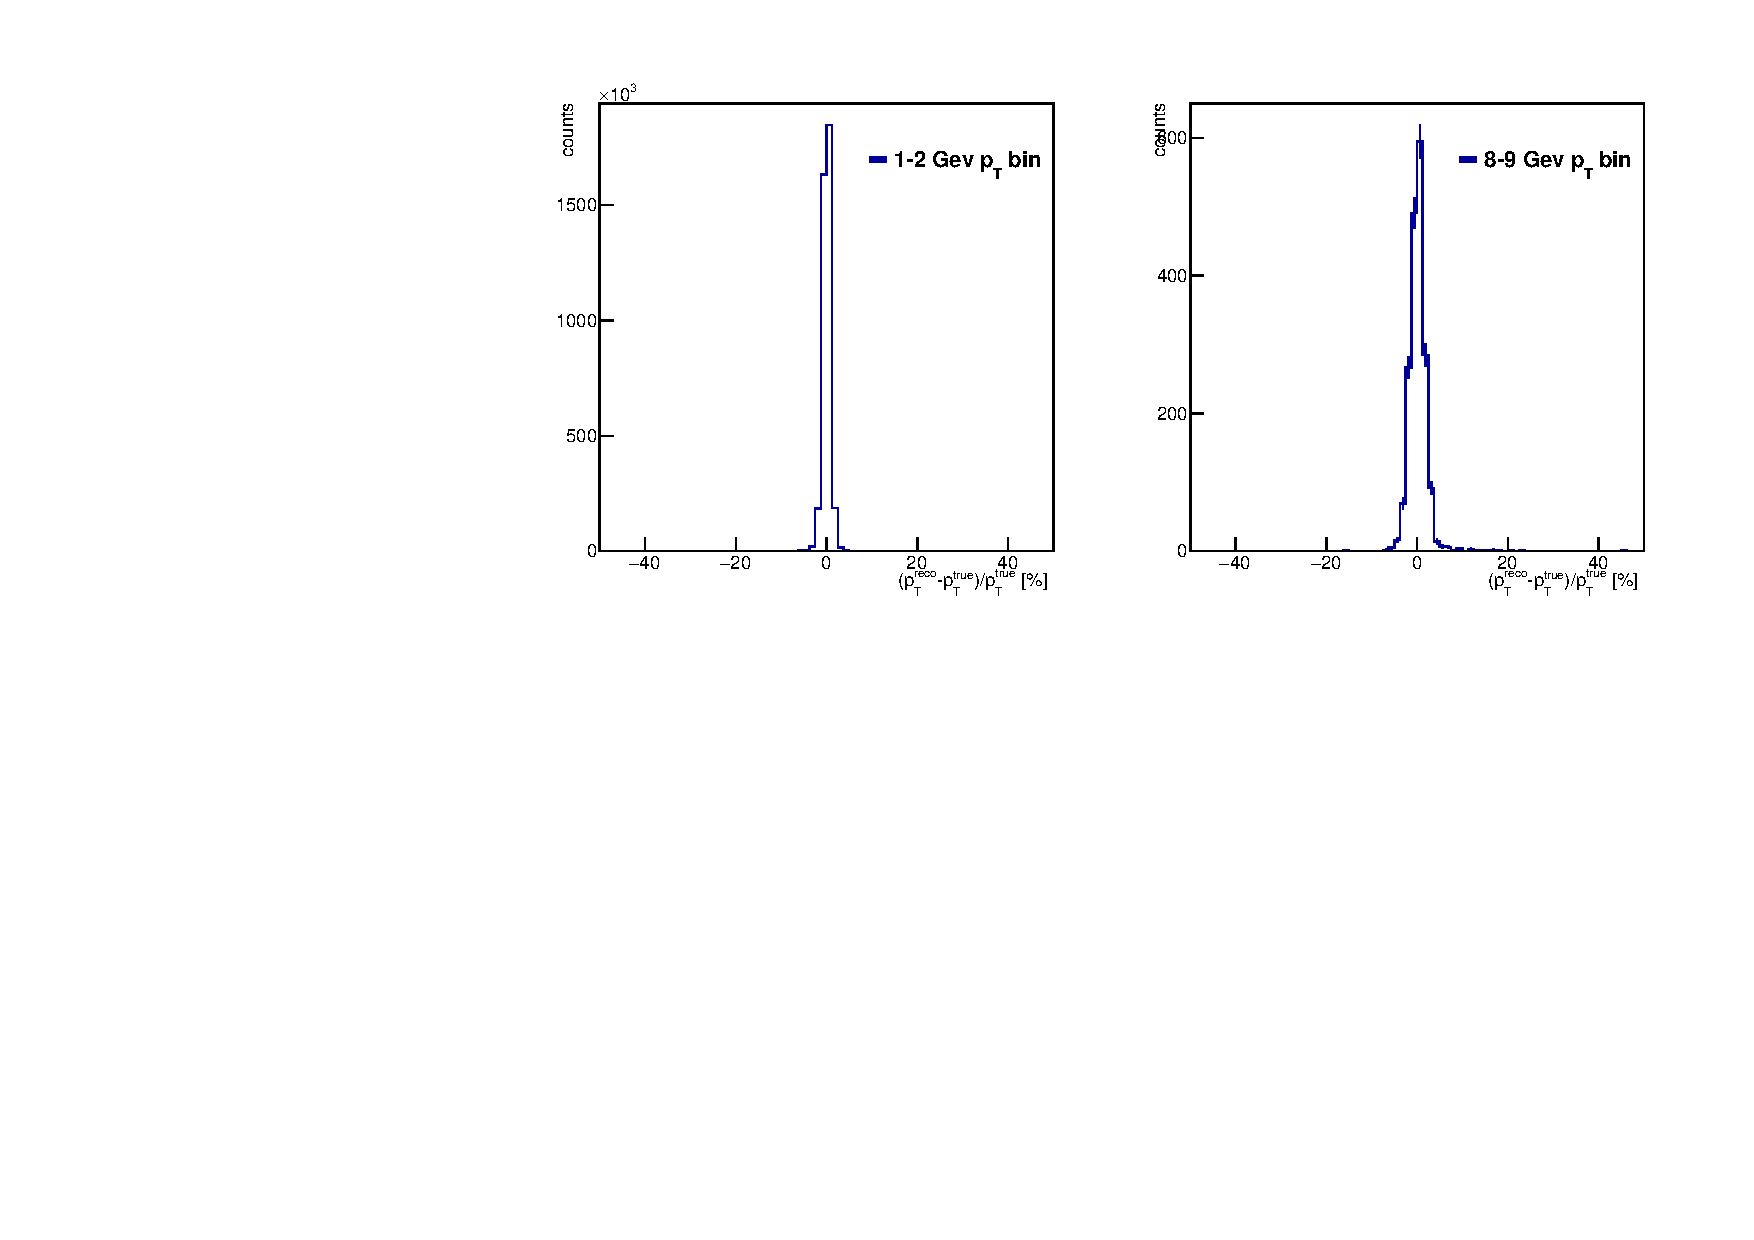
\includegraphics[width=0.95\textwidth]{Data_Analysis/Tracking/gaussianReso_tpc.pdf}
%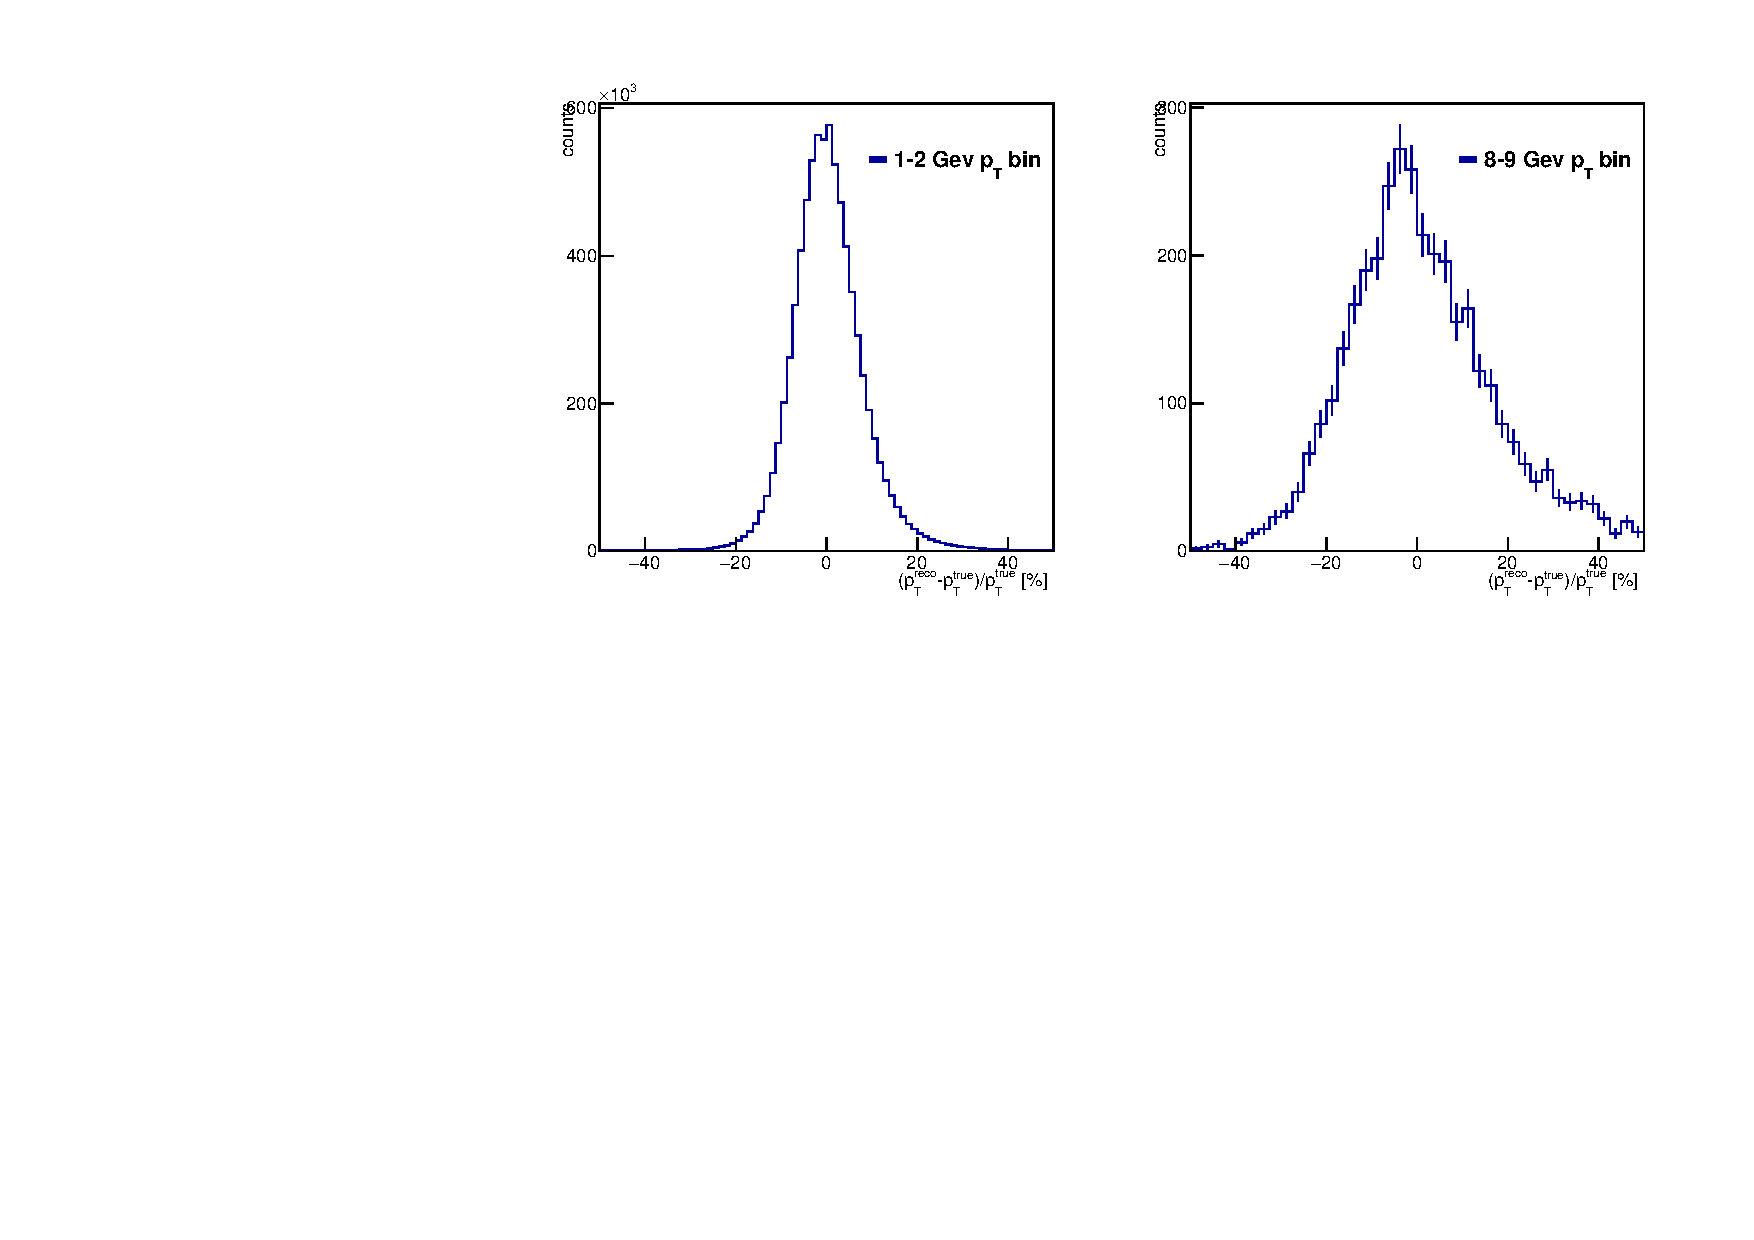
\includegraphics[width=0.95\textwidth]{Data_Analysis/Tracking/gaussianReso.pdf}
%\caption{Relative difference between reconstructed and true momentum for selected intervals of true momentum for TPC+ITS (top) and ITS-only (bottom) using the LHC13b2\_efix\_p1 Monte Carlo simulation. The left panel shows the distribution for 1--2 \GeVc~$\pt^{true}$ range with a standard deviation of 0.84\% for TPC+ITS and 7$\%$ for ITS only, while the right is for the 8--9 \GeVc~$\pt^{true}$ range with a standard deviation of 1.6\% and 15$\%$ respectively.}
%\label{fig:gaussian_reso}
%\end{figure}